\documentclass[a4paper,12pt,twoside]{report}
\usepackage[left=2cm,right=2cm,top=2cm,bottom=3cm]{geometry}


\usepackage[utf8]{inputenc}
\usepackage{amsmath}
\usepackage[spanish, es-tabla]{babel}
\usepackage{amsfonts}
\usepackage{amssymb}
\usepackage{multirow, array} 
\usepackage{chngcntr}
\usepackage{graphicx}
\usepackage{subfig}
\usepackage{cite}
\usepackage{adjustbox}
\usepackage[table]{xcolor}


\usepackage{color}   %May be necessary if you want to color links
\usepackage{hyperref}
\hypersetup{
    colorlinks=true, %set true if you want colored links
    linktoc=page,     %set to all if you want both sections and subsections linked
    linkcolor=blue,  %choose some color if you want links to stand out
}

\title{}
\begin{document}
\begin{center}
\thispagestyle{empty}
\fontsize{12pt}{12pt}\selectfont 

%%%%%%%%%%%%%%%%%%% PORTADA %%%%%%%%%%%%%%%%%%%%%%%%


\textbf {\huge Diseño y calibración de un telescopio de muones híbrido para estudios vulcanológicos.}


\vspace{3cm}

{\large \textbf{Autor:}}

\vspace{0.5cm}

\large Jesús Peña Rodríguez

\vspace{3cm}
{\large \textbf{Director}}\\
\vspace{0.5cm}
{\large Luis A. Núñez}\\
\vspace{0.5cm}
{\large \textbf{Codirector}}\\
\vspace{0.5cm}
{\large Hernán Asorey}
\vspace{3cm}


\normalsize
\large Presentado como requisito del programa de 
\linebreak
\large Doctorado en Ciencias Naturales - Física

\vspace{4cm}

\large Universidad Industrial de Santander\\

\large  Facultad de Ciencias \\

\large  Escuela de Física - Abril 2019
    
  \end{center}
\large


\newpage
%%%%%%%%%% CONTENIDO %%%%%%%

\tableofcontents % indice de contenidos

\cleardoublepage
\addcontentsline{toc}{chapter}{Lista de figuras} % para que aparezca en el indice de contenidos
\listoffigures % indice de figuras


\chapter{Planteamiento del problema}

La muongrafía es una técnica no-invasiva que se utiliza para estudiar grandes estructuras antrópicas o naturales. Sus aplicaciones van desde detección de materiales ocultos en contenedores \cite{Blanpied2015}, arqueología \cite{Morishima2017, Gmez2016, Alvarez1970}, exploración geológica en Marte \cite{Kedar2013}, inspección de plantas nucleares \cite{Fujii2013}, cavidades subterráneas \cite{Saracino2017} y  vulcanología \cite{Tanaka2005, Tanaka2009, Lesparre2010, Lesparre2011, Lesparre2012}.\\

Actualmente las herramientas más utilizadas en el estudio de volcanes son la sismología, gravimetría y tomografía eléctrica. Estas tienen una resolución espacial y capacidad de penetración baja \cite{RosasCarbajal2017}, además los datos deben ser registrados de manera directa sobre la superficie del volcán, \cite{Marteau2012}. La muongrafía ofrece una alternativa con resolución espacial de decenas de metros \cite{Lesparre2012}, una gran capacidad de penetración y la adquisición de información es no-invasiva \cite{Nishiyama2014}.\\

Su funcionamiento se basa en la medición del flujo de muones que cruzan la estructura en diferentes direcciones. Esta medición se hace a través de un hodoscopio\footnote{Instrumento que mide la trayectoria de partículas cargadas haciendo uso de dos o más planos de detección}. Las diferencias de flujo que se proyectan sobre el elemento sensible permiten extraer información de la densidad interna del objeto escaneado.\\

Sin embargo, esta metodología presenta algunos problemas como la sub-estimación de la densidad debido al registro de eventos falso-positivos, los cuales se generan por tres fuentes: los muones horizontales que inciden desde la parte trasera del detector, los muones de baja energía que son dispersados por la superficie del volcán y partículas cargadas procedentes de lluvias aéreas extendidas (EAS) \cite{Nishiyama2014,Gomez2017}.\\

Para reducir estos efectos se han desarrollado diversas técnicas basadas en: la implementación de sistemas de medición del tiempo de vuelo (ToF) para eliminar los muones de albedo\footnote{Muones atmosféricos reflejados hacia la atmósfera por la tierra o generados en ella.)} \cite{Marteau2014, Cimmino2017}, la instalación de paneles absorbentes para filtrar los muones de baja energía y el aumento de la cantidad de paneles sensibles para disminuir la probabilidad de detectar eventos generados por EAS \cite{Lesparre2012}.\\

La instalación de paneles (absorbentes o sensibles) repercute en el aumento de la complejidad del detector. La mejor opción para la eliminación del ruido de fondo son los sistemas ToF y de identificación de partículas. Actialmente, los telescopios MuRay y Diaphane tienen sistemas ToF con resolución de 400 y 240 ps respectivamente \cite{Cimmino2017, Marteau2014}, sin embargo no es suficiente para discriminar los muones y electrones de baja energía.\\

En este trabajo se propone la implementación de un telescopio de muones híbrido capaz de reducir las principales fuentes de ruido que pueden afectar la muongrafía de estructuras volcánicas.

% La principal fuente de ruido en muongrafía son electrones y muones con momento $<$ 1 GeV/c como se reporta en \cite{Nishiyama2014,Gomez2017}.
\chapter{Justificación}

El estudio del interior de grandes estructuras, en especial las geológicas, puede ser realizado a través de muones atmosféricos producidos por rayos cósmicos. El flujo de muones a nivel del mar es $\approx$ 1  muon/cm$^2$min y es capaz de penetrar varios kilómetros de roca \cite{Ariga2018}. La radiografía de muones o muongrafía en estructuras geológicas se hace por medio de un telescopio de muones el cual registra del flujo de muones que atraviesan la estructura en diferentes direcciones. La atenuación del flujo de muones provee información de la distribución de densidad dependiendo de la cantidad del material atravesado.\\

La técnica de la muongrafía fue propuesta por George en 1955 \cite{George1955} e implementada inicialmente por Alvarez en 1970 \cite{Alvarez1970}. Actualmente se utiliza en diversas áreas, siendo la geología la más representativa. En este campo se han realizado trabajos de muongrafía de volcanes \cite{Tanaka2009, Lesparre2012, Carbone2013}, cavernas \cite{Saracino2017, Olh2013}, acuíferos \cite{Jourde2016}, reservorios de CO2 \cite{Zhong2015, Klinger2015, Zhong2016} y glaciares \cite{Nishiyama2017, Ariga2018}.\\

En años recientes los esfuerzos se han centrado en el refinamiento de la técnica para estudiar estructuras geológicas, abordando temas como el ruido de fondo generado por los muones de baja energía \cite{Nishiyama2014,Gomez2017}, el ruido causado por la componente electromagnética de la lluvias aéreas de partículas \cite{KUSAGAYA2015, Nishiyama2014Noise, Marteau2012Noise}, los efectos de la composición de la roca sobre la muongrafía \cite{Lechmann2018}, el aumento de su eficiencia mediante sistemas ToF \cite{Shi2014} y su viabilidad para hacer estudios del comportamiento dinámico de estructuras geológicas\cite{Jourde2016}.\\

Un telescopio de muones que reduzca el ruido fondo debe tener tres características:

\begin{itemize}
    \item Identificar y filtrar los muones de baja energía ($<$ 1 GeV) causantes de la mayor parte de ruido de fondo. 
    \item Identificar los $e^{\pm}$ y $\gamma$ generados por lluvias aéreas que pueden emular la trayectoria que trazaría un muón proveniente del volcán. 
    \item Identificar y filtrar los muones que atraviesan el telescopio desde la parte trasera del detector.
\end{itemize}

La eliminación de eventos falsos mejora la estimación de la densidad de la estructura escaneada a partir del flujo de muones emergente.\\

En este proyecto se propone el desarrollo y calibración de un telescopio de muones que estime las diferencias de densidades de una estructura teniendo en cuenta las fuentes de ruido anteriormente expuestas.






















\chapter{Objetivos}
\section{\textbf{Objetivo General}}

Diseñar, construir y calibrar el sistema electrónico de un telescopio de muones para el estudio de estructuras geológicas capaz de filtrar las principales fuentes de ruido encontradas en la muongrafía hasta la fecha.

\section{\textbf{Objetivos Específicos}}

\begin{itemize}
    \item Diseñar y calibrar el sistema electrónico de un hodoscopio que permita registrar el flujo de muones en diferentes direcciones.
    
    \item  Implementar un sistema ToF de alta resolución temporal capaz de discriminar los muones con momento $< 1$ GeV y los muones de albedo.

    \item  Diseñar y calibrar el sistema electrónico de un subdetector (WCD) que ayude a diferenciar los $\mu^{\pm}$ de los $e^{\pm}$ y $\gamma$ generados por lluvias aéreas extendidas (EAS).
    
    %\item Calibrar el hodoscopio con el fin de obtener una respuesta uniforme en cada uno de sus píxeles y obtener una reconstrucción confiable del flujo de muones.
    
    %\item Calibrar el WCD para obtener el punto óptimo de operación que maximice la discriminación entre  $\mu^{\pm}$ y $e^{\pm}, \gamma$.
    
    %\item Acoplar el hodoscopio y el WCD en un sistema conjunto de adquisición que sea robusto e independiente.
    
    \item Validar el desempeño del Telescopio de Muones (MuTe) en la reducción del ruido en muografía. 
    
    %\item Instalar sistemas periféricos que suministren información acerca del funcionamiento del detector.
    
    %\item Hacer un análisis detallado de las principales fuentes de ruido en la muongrafía a partir de los datos recolectados.
    
\end{itemize}
\chapter{Estado del arte}

\label{ch:background}

\section{Rayos cósmicos primarios}

Los rayos cósmicos (CR) fueron identificados por primera vez en 1912 por Victor Hess. Hess encontró que la radiación aumentaba considerablemente con la altura y concluyó que tenía origen extraterrestre. Los CR primarios son partículas que viajan a través del espacio hasta interactuar con la atmósfera terrestre generando cascadas de partículas secundarias.\\

El flujo de primarios que llega a la Tierra son 90$\%$ protones, 9$\%$ núcleos de helio y 1$\%$ iones pesados, electrones y otros \cite{Spurio2015}. El origen de los RC primarios depende de su energía, $E$. La mayoría de los CR con $E<10^{10}$ eV provienen del viento solar, para energías $10^{10}$ eV $ < E <$ $10^{18}$ eV el origen más probable es galáctico, en particular de remanentes de supernovas y para $E>10^{18}$ eV la fuente es extragaláctica \cite{Procureur2018}. Recientemente, el observatorio Pierre Auger confirmó que los CR de Ultra Alta Energía (UHECR por sus siglas en inglés) ($> 10^{18}$ eV) proceden de fuera de nuestra galaxia \cite{Pierre2017}.\\

El espectro, $\Phi$, de los CR que ingresan a nuestro planeta se representa con la ley de potencia:

\begin{equation}
  \frac{d \Phi}{dE}  = A \cdot E^{- \alpha} 
\end{equation}
donde $A$ es la normalización respecto al eje \textit{y} y $\alpha$ es el índice espectral diferencial. 
Usualmente el flujo es multiplicado por una potencia de energía, $E^\beta$, para evidenciar ciertas estructuras en el espectro que marcan puntos importantes en el entendimiento del origen de los CR.

\begin{equation}
E^\beta \cdot \frac{d \Phi}{dE}  =   A \cdot E^{- \alpha + \beta}
\end{equation}

\begin{figure}[h!]
\begin{center}
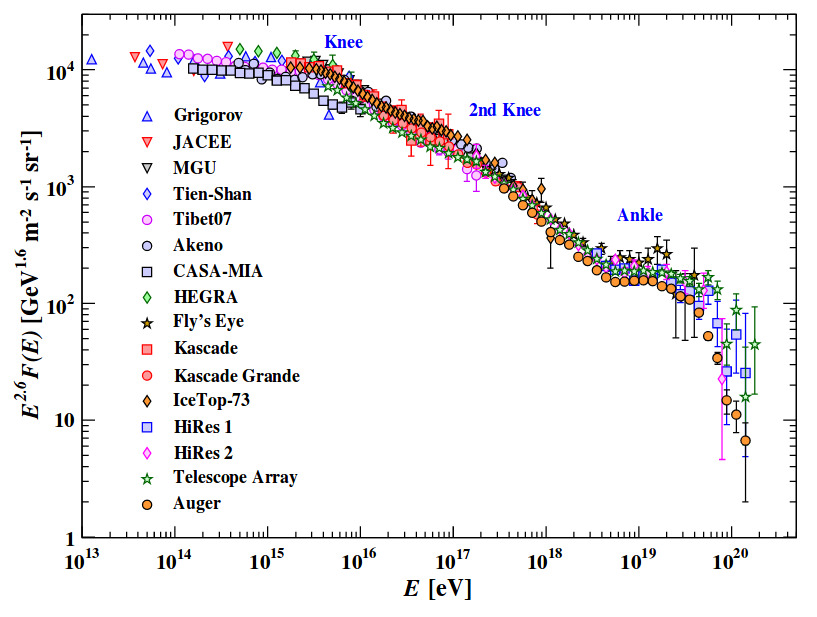
\includegraphics[width=0.9\textwidth]{Figures/Flux}
\caption[Flujo diferencial de CR en función de la energía.]{Flujo diferencial de CR en función de la energía. Los datos de flujo son obtenidos de manera directa o de indirecta por diferentes observatorios (izquierda). Para resaltar las estructuras de la \textit{rodilla} y el \textit{tobillo} se toma un $\beta = 2.6$ \cite{Spurio2015}.}
\label{Flux}
\end{center}
\end{figure}

La caracterización del espectro del flujo de CR se realiza mediante mediciones hechas por diferentes experimentos como se muestra en la Fig. \ref{Flux}. En el espectro se pueden observar dos estructuras particulares asociadas con los cambios de pendiente del espectro. La llamada \textit{rodilla}, alrededor de $10^{15}$ eV, representa una transición entre diferentes clases de mecanismos galácticos de aceleración de CR y de la capacidad de aceleración de las fuentes galácticas. Por otra parte, existe un punto de cambio de pendiente llamado \textit{tobillo} ($\sim 10^{18}$ eV) a partir del cual comienza el flujo de CR de origen extragaláctico, \cite{Spurio2015}.

\section{Partículas secundarias}

Cuando los CR entran a la atmósfera terrestre iteractúan con los núcleos que la componen, produciendo gran cantidad de partículas secundarias (bariones, mesones y leptones). Dependiendo de su tiempo de vida estas partículas pueden interactuar nuevamente o decaer, y generan un efecto cascada llamada lluvia aérea extendida (EAS por sus siglas en inglés). Particularmente, los mesones cargados, típicamente piones y kaones, pueden decaer en muones, electrones y neutrinos, y los piones neutros decaen en fotones.

\begin{figure}[h!]
\begin{center}
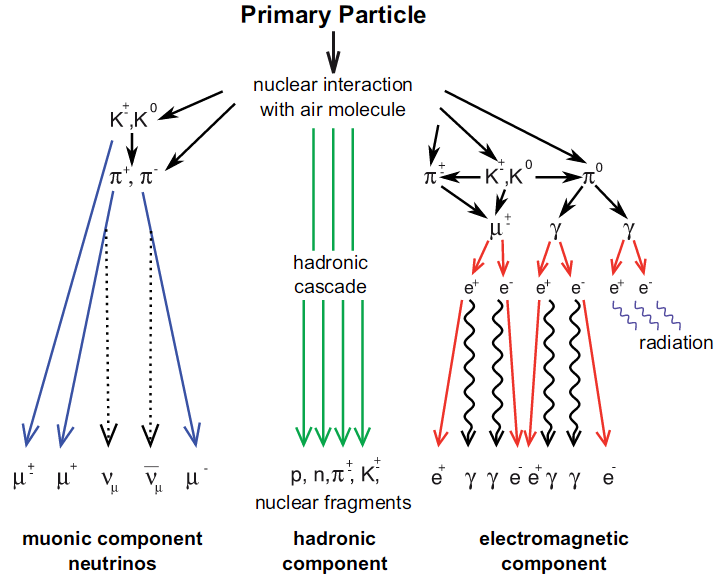
\includegraphics[width=0.7\textwidth]{Figures/EAS_Components}
\caption[Componentes de la lluvia aérea extendida]{La interacción del CR primario con los átomos de la atmósfera genera un chubasco de partículas secundarias compuesto por una parte hadrónica (verde), una electromagnética (roja) y una muónica (azul\textbf{}), \cite{Haungs2011}.}
\label{Components}
\end{center}
\end{figure}

Las EAS tienen tres componentes: la \textbf{electromagnética}, compuesta por fotones, electrones, positrones y usualmente neutrinos electrónicos, la \textbf{hadrónica} compuesta por kaones, piones, neutrones y protones y la componente \textbf{muónica} compuesta por muones y neutrinos muónicos, Fig. \ref{Components}.

El desarrollo longitudinal y lateral de la EAS depende de la energía del CR primario que la genera como se muestra en la Fig. \ref{EAS}. Además, el número total de partículas generado en una EAS se relaciona con el ángulo de incidencia del primario y la altura a la cual ocurrió la primera interacción \cite{Grieder2010}.

\begin{figure}[h!]
\begin{center}
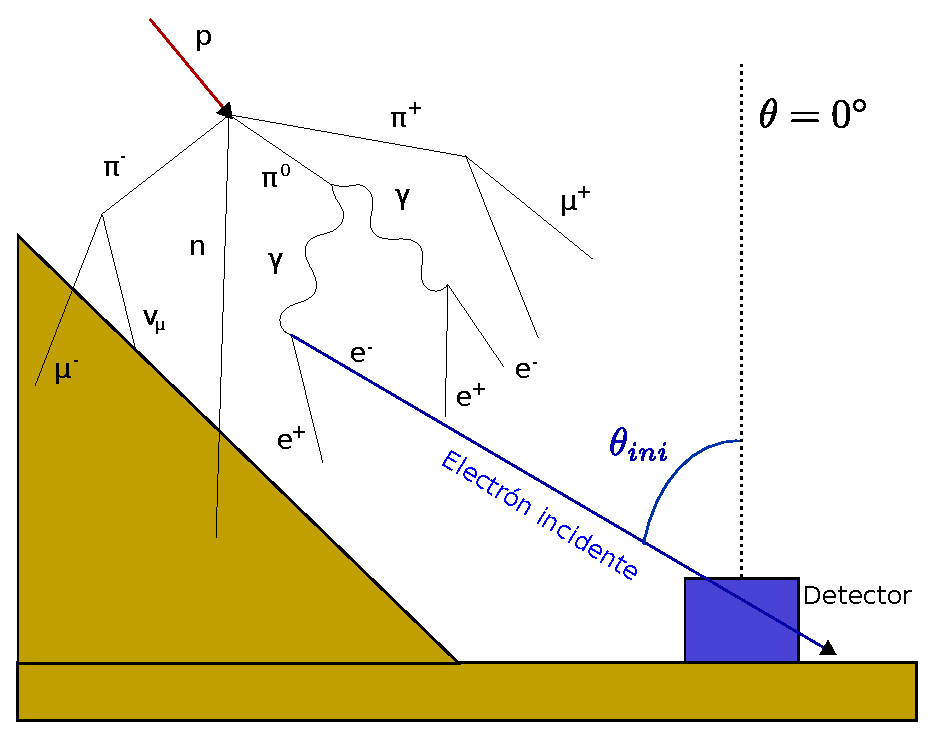
\includegraphics[width=0.5\textwidth]{Figures/EAS}
\caption[Desarrollo longitudinal de una EAS en la atmósfera]{Desarrollo longitudinal de una EAS en la atmósfera. En este caso, se muestra el tamaño de la lluvia en función de la profundidad atmosférica, $X$, para diferentes energías del primario ($E_1<E_2<E_3<E_4$) \cite{Grieder2010}. La profundidad atmosférica se define como la integral en la dirección del primario de la densidad atmosférica sobre el punto de observación.}
\label{EAS}
\end{center}
\end{figure}

\section{Componente muónica}

Las dos fuentes principales de producción de muones corresponden al decaimiento de los kaones $K^{\pm}$ y los piones $\pi^{\pm}$. En el caso de los kaones $K^+$, aproximadamente el $90\%$ de decaimientos ocurre en tres canales \cite{Olive2014}:
\begin{equation}
\begin{array}{ll}
K^+ \rightarrow \mu^+ + \nu_{\mu} & 63.56\% \\
K^+ \rightarrow \pi^+ + \pi^0 & 20.67\% \\
K^+ \rightarrow \pi^+ + \pi^+ + \pi^- &5.58\%
\end{array}
\end{equation}

Para los piones $\pi^\pm$ el $99.9\%$ de los decaimientos ocurren en el canal \cite{Olive2014}:
\begin{eqnarray}
\pi^+ \rightarrow \mu^+ + \nu_{\mu}\\
\pi^- \rightarrow \mu^- + \bar{\nu}_{\mu}
\end{eqnarray}
La componente muónica es la más penetrante de las tres y puede sobrevivir hasta alcanzar la superficie terrestre, debido a dos factores:

\begin{itemize}
\item Un tiempo de vida de $2.2 \times 10^{-6}$ s, el cual es dos órdenes de magnitud mayor a los mesones  $\pi^{\pm}$ $(2.6 \times 10^{-8}$ s) o los $K^{\pm}$ $(1.23 \times 10^{-8}$ s). Debido a su alta energía, los muones pueden desplazarse grandes distancias en la atmósfera sin decaer, $L($km$) = 6200\times E($TeV), \cite{Procureur2018, Nagamine2003}. 

\item Una masa de 105.5 MeV/c$^2$ la cual es $\approx200$ veces mayor que la del electrón. La pérdida de energía por \textit{Bremsstrahlung} es proporcional a $1/m^2$, siendo menor para muones que para electrones a una energía dada. Los muones pierden energía mayormente por ionización hasta energías del orden de 1 TeV en el aire \cite{Groom2001}.

\end{itemize}

\section{Muónes atmosféricos como fuente de radiación}


El estudio de grandes estructuras mediante muongrafía se basa en el principio de la \textit{radiografía}, es decir, la radiación a la que se expone un objeto es absorbida parcialmente dependiendo de su densidad. Para estimar la diferencia de densidad en una determinada trayectoria se usa un elemento sensor ubicado en el lado opuesto del objeto con el fin de medir el flujo de partículas capaces de atravesarlo y el conocimiento previo de su geometría. 

\begin{figure}[h!]
\begin{center}
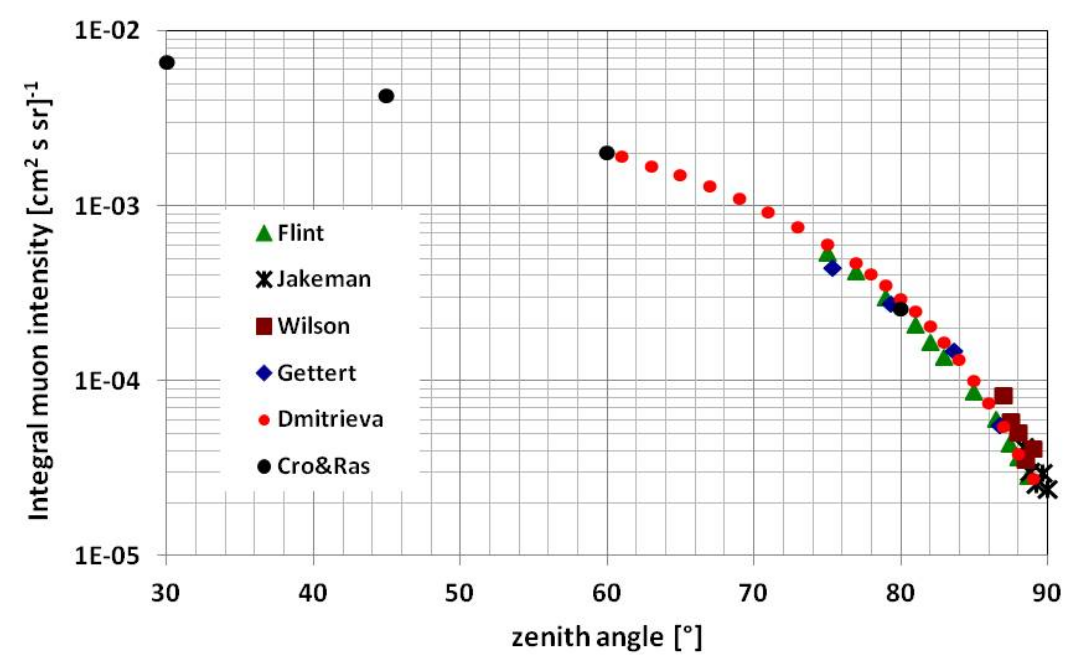
\includegraphics[width=0.8\textwidth]{Figures/Muon_flux}
\caption[Variación del flujo integral de muones a nivel del mar dependiendo del ángulo zenital]{Variación del flujo integral de muones a nivel del mar dependiendo del ángulo zenital. Los puntos corresponden a los experimentos: Flint et al. (1972), Jakeman (1956), Wilson (1959), Gettert et al. (1993), Dmitrieva et al. (2006), Crokes and Rastin (1972) \cite{Cecchini2012}.}
\label{Muon_flux}
\end{center}
\end{figure}

Teniendo en cuenta la analogía anterior, la muongrafía utiliza como fuente de radiación los muones atmosféricos creados por la interacción de los rayos cósmicos con los núcleos de los átomos que componen la atmósfera terrestre. Esta interacción causa un flujo de partículas constante en el tiempo, pero, dependiente del ángulo de observación respecto al cenit, $\theta$. El número partículas que logran alcanzar el suelo terrestre en la dirección vertical es mayor en comparación con la dirección horizontal, debido a que el espesor de la atmósfera terrestre es menor en $\theta=0^o$. Este comportamiento se puede modelar mediante la función $\cos^2 \theta$ como se muestra en la Fig. \ref{Muon_flux}.

\section{Radiografía de muones}

Esta técnica hace uso de la atenuación del flujo de muones en una trayectoria determinada debido a la pérdida de energía por su interacción con el material.\\

Los muones atmosféricos, con una energía cinética entre $\sim 0.1$ GeV y $\sim 100$ GeV, pueden atravesar grandes cantidades de roca estándar ya que en esta región se comportan como partículas de mínima ionización (MIP por sus siglas en inglés), es decir, la pérdida de energía $dE/d\text{x}$ por su interacción con la materia ocurre mayoritariamente por ionización. Por otro lado, los muones con energía cinética $> 693$ GeV pierden energía principalmente por efecto del \textit{Bremsstrahlung} (radiación de frenado) y para  $< 693$ GeV las pérdidas ocurren mayormente debido a la ionización. Ver Fig. \ref{Stopping_Power}.

%\begin{figure}[h!]
%\begin{center}
%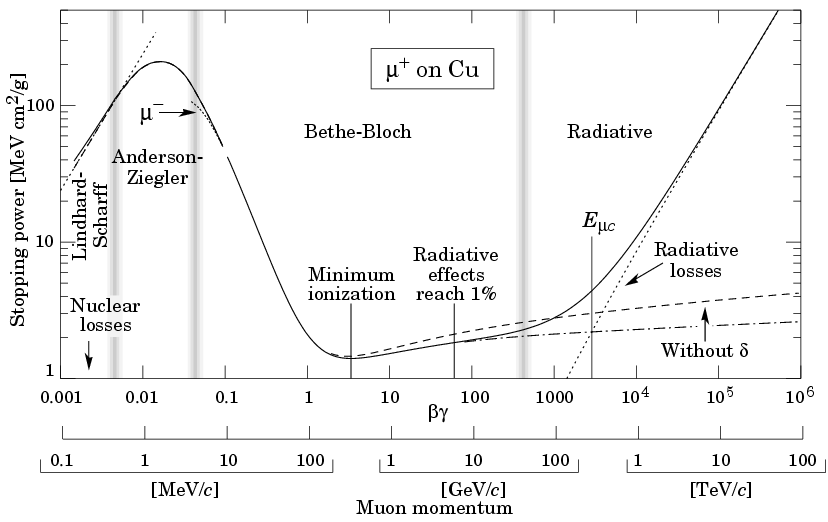
\includegraphics[width=1\textwidth]{Figures/Bethe_Block}
%\caption[Pérdida de energía para muones positivos en cobre como función del cantidad de movimiento]{Pérdida de energía para muones positivos en cobre como función del cantidad de movimiento. La $-dE/dx$ para muones es dominada por tres efectos: la pérdida por interacción con los núcleos y electrones atómicos (0.1-100 MeV/c), la pérdida por ionización (1-100 GeV/c) y la pérdida por radiación (1-100 TeV/c) \cite{Agashe2014}.}
%\label{Stopping_Power}
%\end{center}
%\end{figure}

\begin{figure}[h!]
\begin{center}
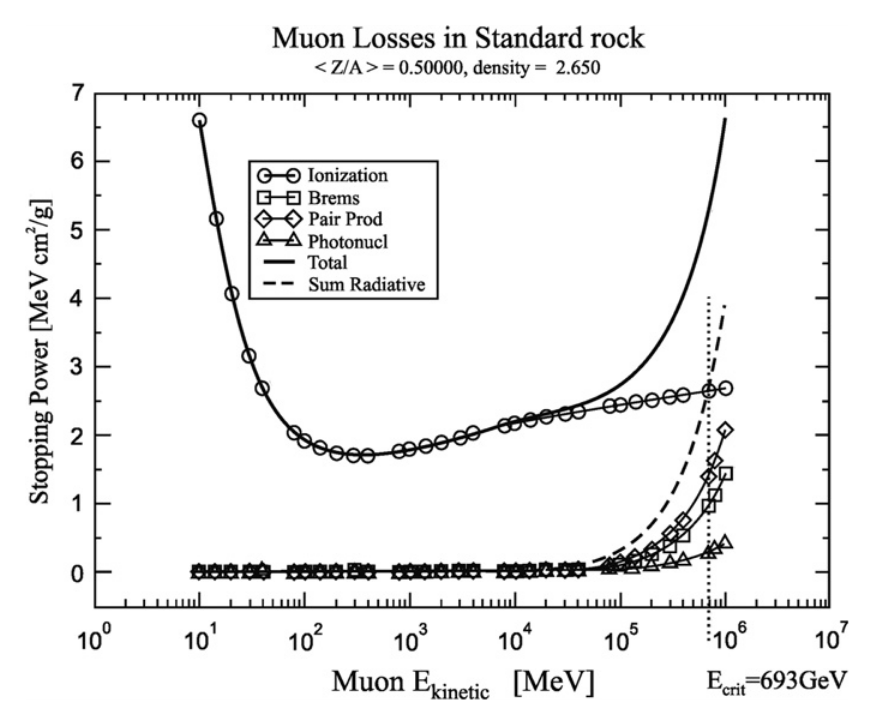
\includegraphics[width=0.8\textwidth]{Figures/Stopping.png}
\caption[Pérdida de energía para muones en roca estándar como función de la energía cinética]{Pérdida de energía para muones en roca estándar como función de la energía cinética. La $-dE/dx$ para muones es dominada por tres efectos: la pérdida por interacción con los núcleos y electrones atómicos ($<$ 0.01 GeV), la pérdida por ionización (0.01-693 GeV) y la pérdida por radiación ($>$ 693 GeV) \cite{Annunziata2012, Groom2001}}
\label{Stopping_Power}
\end{center}
\end{figure}

%La pérdida de energía es modelada por la fórmula de Bethe-Bloch:

%\begin{equation}
%-\frac{dE}{dx} = Kz^2\frac{Z}{A}\frac{1}{\beta^2} \left[ \frac{1}{2} \ln  %\frac{2m_ec^2\gamma^2\beta^2}{I^2}T_{max} - \beta^2 -\frac{\delta}{2}\right]
%\end{equation}
%con
%\begin{equation}
%K=4\pi N_Ar_e^2m_ec^2=0.307MeVg^{-1}cm^2
%\end{equation}

%donde, $z$ es la carga de la partícula incidente, $Z$ es el número atómico del material, $A$ es la masa del material, $\beta$ es la velocidad de la partícula incidente, $m_e$ es la masa del electrón, $\gamma$ es el factor de Lorentz, $T_{max}$ es la energía máxima transferida en una colisión, $I$ es la energía de excitación media en el material, $\delta$ es una corrección de densidad, $N_A$ el número de Avogadro y $r_e$ es el radio clásico del electrón el cual se define como:

%\begin{equation}
%    r_e =\frac{1}{4\pi \epsilon_0}\frac{e^2}{m_e c^2}
%\end{equation}

%donde $e$ carga eléctrica del electrón y $\epsilon_0$ es la permitividad del vacío.

\begin{figure}[h!]
\begin{center}
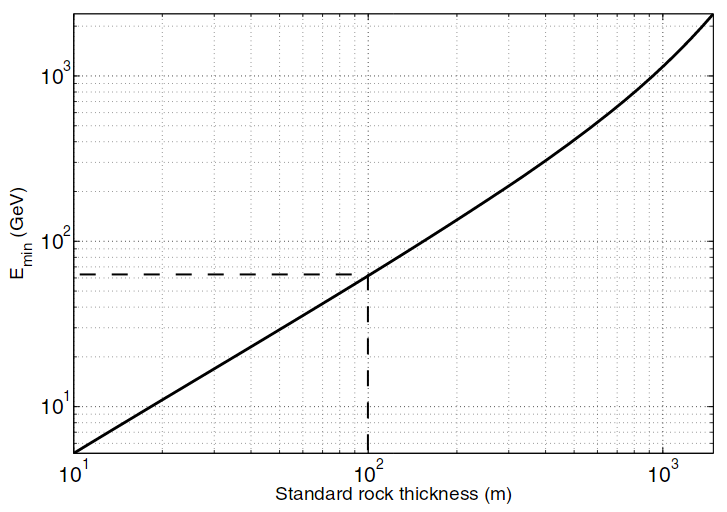
\includegraphics[width=0.7\textwidth]{Figures/Min_Energy}
\caption[Energía mínima requerida por un muón para cruzar una longitud $L$ de roca estándar cuya densidad es $\rho = 2.65 \ g/cm^3$]{Energía mínima requerida por un muón para cruzar una longitud $L$ de roca estándar cuya densidad es $\rho = 2.65$ g/cm$^3$ \cite{Catalano2016, Lesparre2010, Valencia2016, Vesga2018}.}
\label{E_min}
\end{center}
\end{figure}

Los muones deben tener una energía mínima $E_{min}$ que les permite atravesar una determinada cantidad de material sin ser absorbidos por el medio.
 En el caso de estudio de estructuras volcánicas, se toma como referencia un medio conformado por roca estándar cuya densidad es $\rho = 2.65$ g/cm$^3$. Por ejemplo, un muón debe tener una energía mínima $\approx 60 \ GeV$ para atravesar una distancia de 100 m de roca estándar, tal y como se ilustra en la Fig. \ref{E_min}.

%########### Hodoscopios ###################

\section{Hodoscopios}

La muongrafía requiere un sistema de detección capaz de medir el flujo de muones dependiendo de la trayectoria como se muestra en la Fig. \ref{Hodoscopio}. Un hodoscopio (``hodos'' + ``skopos'' = trayectoria + observador) es un instrumento que registra la trayectoria de partículas cargadas haciendo uso de dos o más planos matriciales en los cuales se determina la posición de la partícula interactuante. El flujo de muones en determinada dirección se estima mediante el conteo de eventos por unidad de tiempo.\\

Además de medir la dirección del flujo de muones, los hodoscopios pueden proveer información adicional de las partículas como el tiempo de vuelo (ToF).\\

\begin{figure}[h!]
\begin{center}
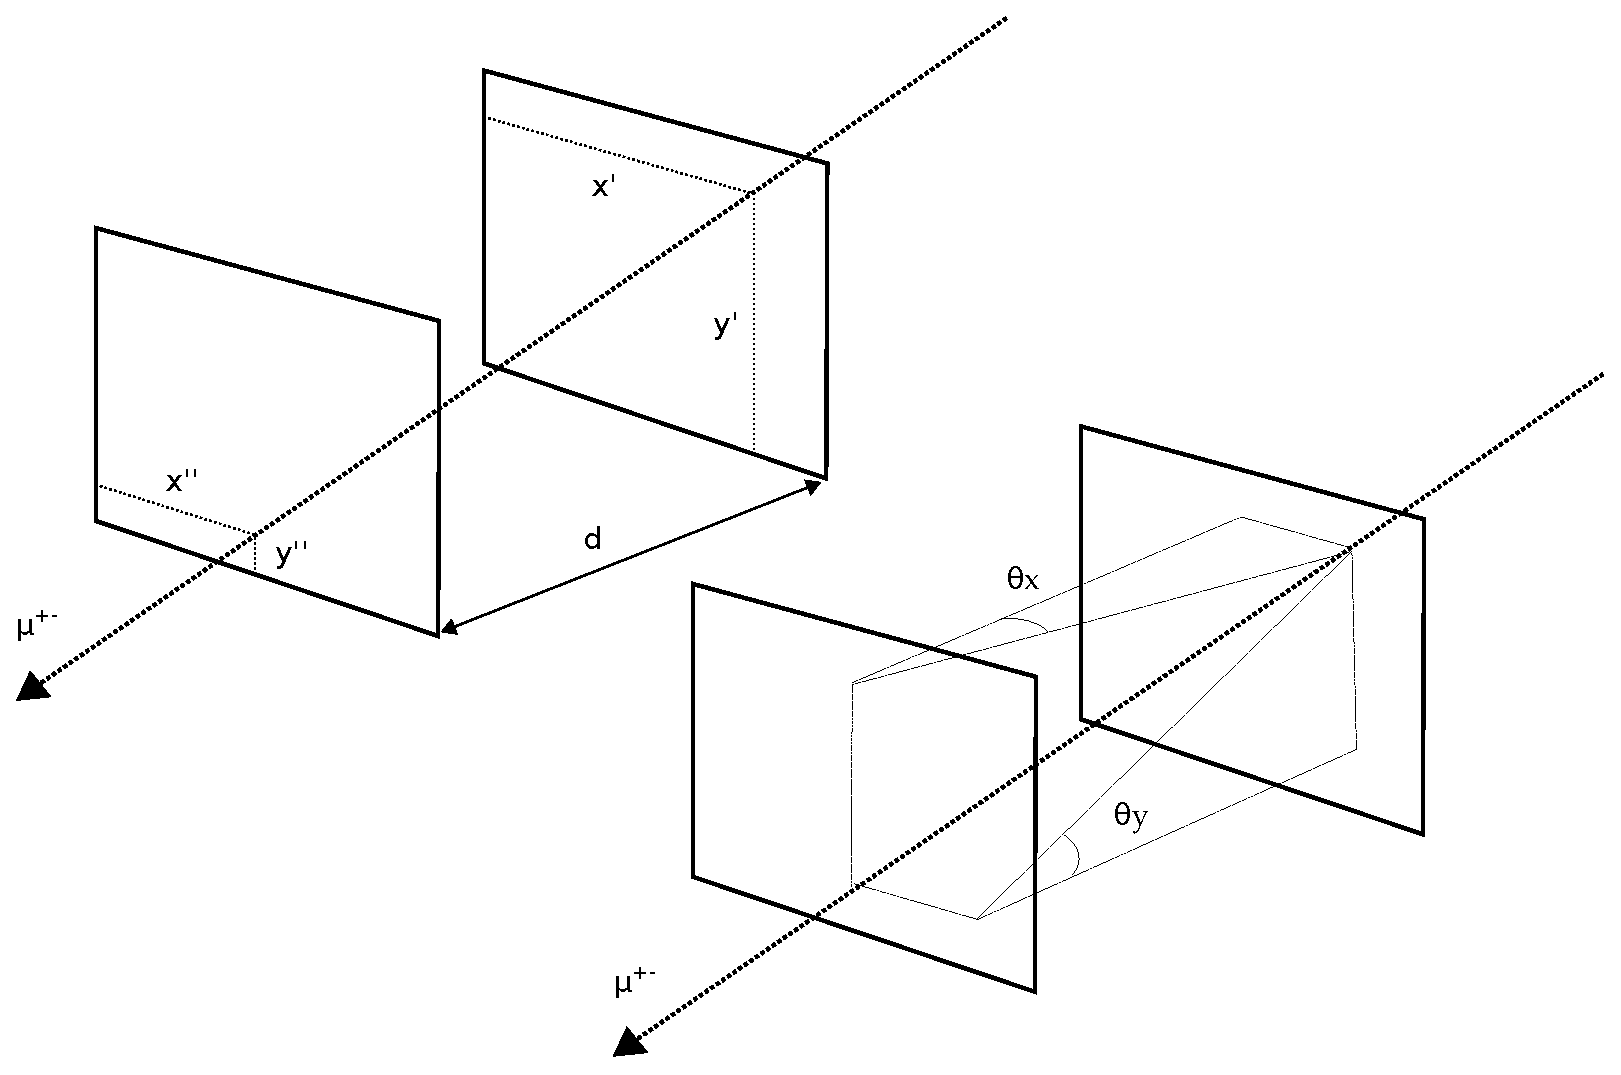
\includegraphics[width=0.8\textwidth]{Figures/Hodoscopio}
\caption[Principio de funcionamiento de un hodoscopio]{Principio de funcionamiento de un hodoscopio. El detector se conforma de al menos dos paneles, cada uno de los cuales mide la posición al paso de un muón $(x',y')$ por el panel frontal y $(x'',y'')$ por el panel trasero, luego se calcula su trayectoria en términos de los ángulos $\theta_x=\tan^{-1} (x^\prime - x^{\prime\prime})/d$ y $\theta_y=\tan^{-1} (y^\prime - y^{\prime\prime})/d$.}
\label{Hodoscopio}
\end{center}
\end{figure}

Finalmente, los paneles sensibles de un hodoscopio se basan en diferentes clases de detectores: centelladores segmentados \cite{Fujii2013, Lesparre2012, Tanaka2009}, centelladores contínuos \cite{Nagamine1995, Aguiar2015, Tang2016}, Cámaras de Plato Resistivo (RPC) \cite{Sehgal2016, Fehr2012}, Micromegas \cite{Bouteille2016}, Cámaras Proporcionales Multi-Hilo (MWPC) \cite{Olh2018} y láminas de emulsión \cite{Morishima2017, NAGAMINE2016}. Cada uno de éstos tiene ventajas y desventajas respecto a la resolución espacial, temporal, robustez mecánica, adquisición de la información y costo.\\

Los detectores anteriores se basan principalmente en tres técnicas de detección: centelladores plásticos (continuos y segmentados), emulsiones nucleares (láminas de emulsión) y detectores gaseosos (RPCs, MWPCs, Micromegas).

\subsection{Centelladores plásticos}

Los centelladores basan su principio de detección en el proceso de excitación y des-excitación de los electrones atómicos del material plástico cuando una partícula cargada lo atraviesa \cite{Grupen2008, Kleinknecht2005}.\\

Los fotones generados por la des-excitación son guiados, a través de una fibra óptica de corrimiento de longitud de onda (WLS), hasta el dispositivo sensor (tubo fotomultiplicador - PMT o fotomultiplicador de silicio - SiPM) como se ilustra en la Fig. \ref{Scintillator}. La fibra WLS tiene un desfase entre sus longitudes de onda de absorción y de emisión, lo cual le permite acoplar eficientemente el espectro de emisión del centellador y el espectro de absorción del elemento sensor. Ver la Fig. \ref{WLS}.

\begin{figure}[h!]
\begin{center}
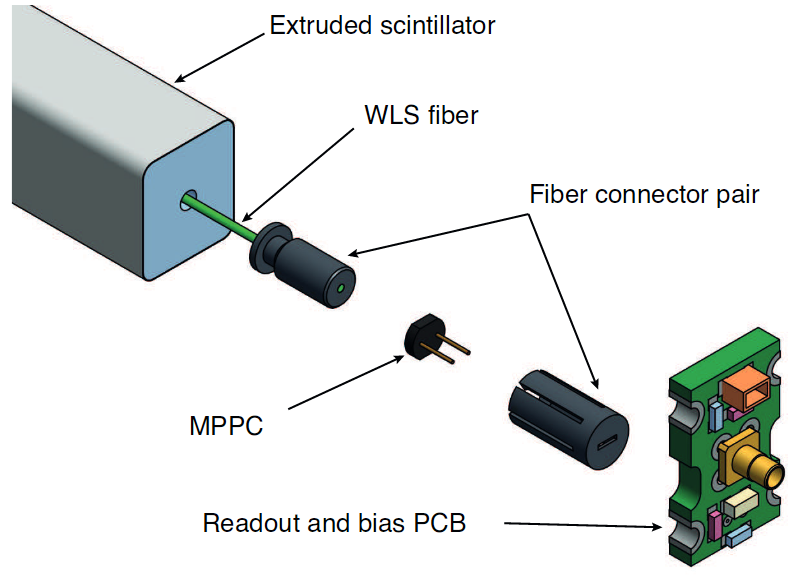
\includegraphics[width=0.55\textwidth]{Figures/Scintillator}
\caption[Sistema de conexión típico entre un centellador segmentado, una fibra óptica WLS y un foto-sensor]{Sistema de conexión típico entre un centellador segmentado, una fibra óptica WLS y un foto-sensor \cite{Str2014}.}
\label{Scintillator}
\end{center}
\end{figure}

\begin{figure}[h!]
\begin{center}
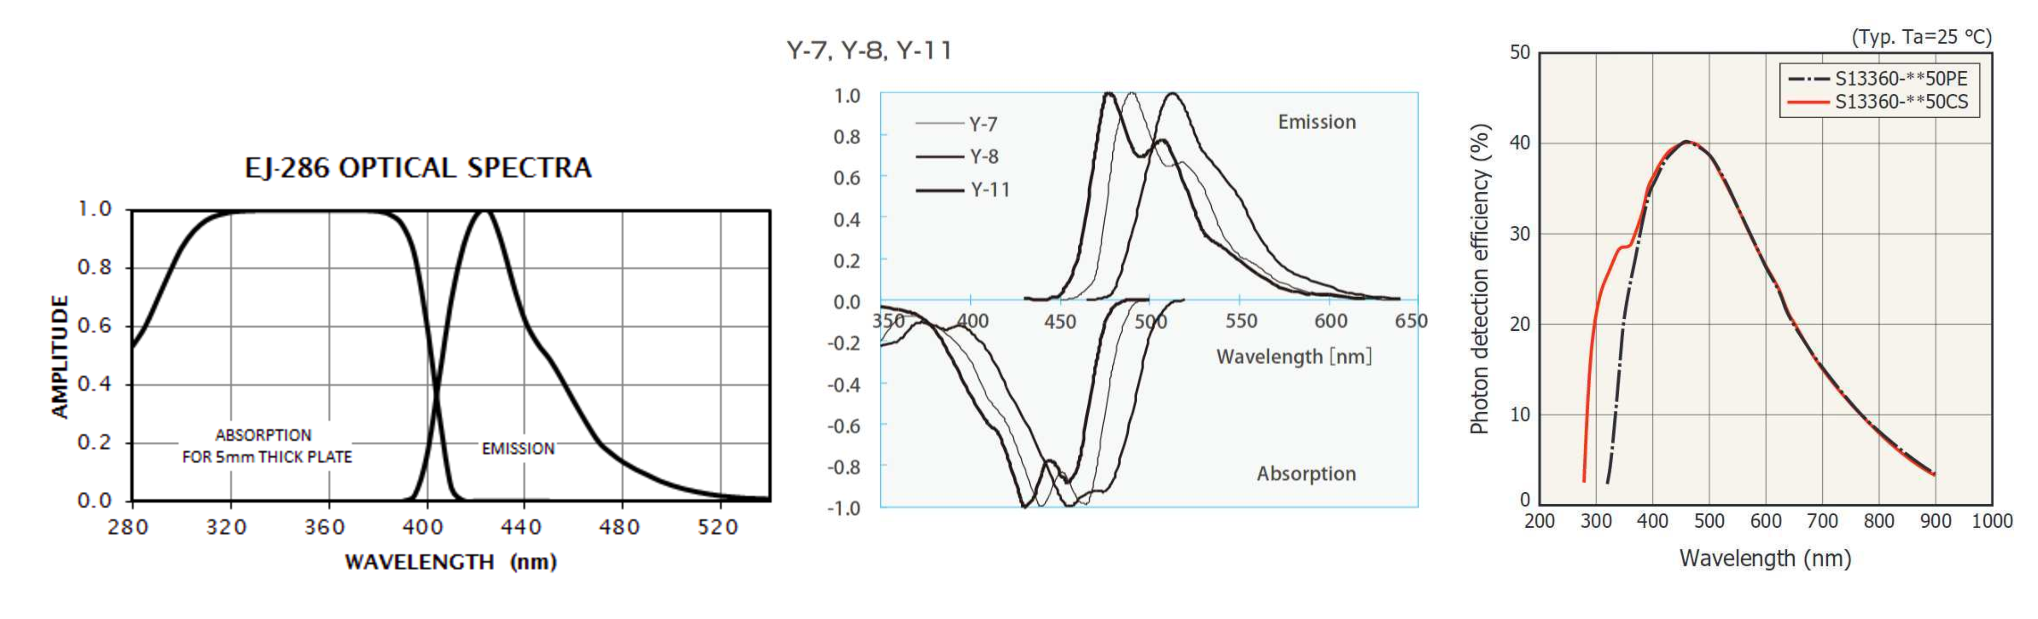
\includegraphics[width=1\textwidth]{Figures/WLS}
\caption[Espectros de absorción y emisión para una barra centelladora EJ-286 de ELJEN Technology, para tres WLS (Y-7, Y-8, Y-11) de Kurarayy el SiPM S13360-50CS de Hamamatsu ]{Espectros de absorción y emisión para una barra centelladora EJ-286 de ELJEN Technology \cite{Eljen2016}, para tres WLS (Y-7, Y-8, Y-11) de Kuraray \cite{Kuraray2018} y el SiPM S13360-50CS de Hamamatsu \cite{Hamamatsy2018}. El máximo de emisión del centellador es 430 nm y el de eficiencia del SiPM es 490 nm.}
\label{WLS}
\end{center}
\end{figure}

Los detectores de centelleo son robustos, fáciles de construir, relativamente económicos, insensibles a las condiciones ambientales y con una alta eficiencia de detección. Su principal desventaja es la resolución espacial. La cual es definida por la desviación estándar de una distribución uniforme, $w/\sqrt{12}$, donde $w$ es el ancho del centellador, \cite{Procureur2018}. 

\subsection{Emulsiones nucleares}

La técnica de emulsiones nucleares se basa en el principio de funcionamiento de la fotografía análoga. Cristales de haluro de plata son mezclados en una gelatina y revestidos sobre un sustrato de vidrio. La interacción de los haluros con los muones desencadena un proceso de oxido-reducción que los convierte en plata metálica \cite{Procureur2018}. Después de la exposición los haluros de plata restantes son disueltos dejando una cubierta negra sobre la posición de los muones, como se ve en la Fig. \ref{Emulsion} .  

\begin{figure}[h!]
\begin{center}
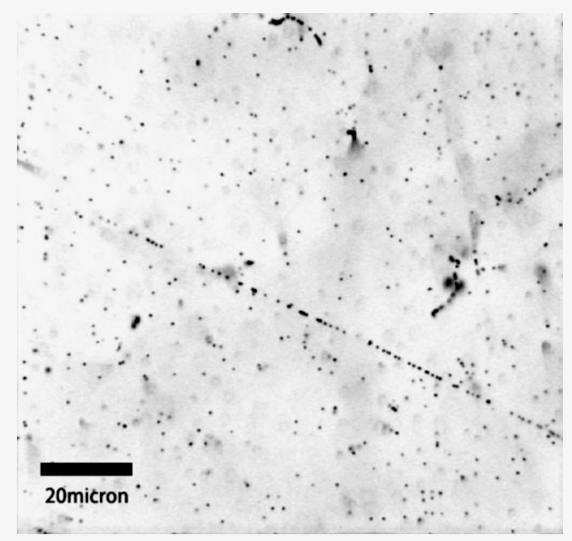
\includegraphics[width=0.45\textwidth]{Figures/Emulsion}
\caption[Imagen microscópica de la trayectoria de un muón (línea punteada) en una lámina de emulsión]{Imagen microscópica de la trayectoria de un muón (línea punteada) en una lámina de emulsión \cite{Nishiyama2014}.}
\label{Emulsion}
\end{center}
\end{figure}

Las láminas de emulsión tienen una alta resolución espacial ($\sim$ $\mu$m) y no consumen energía, sin embargo, el tiempo de vida de las láminas es corto ($\sim$ meses) y depende de la humedad y temperatura del ambiente en el cual se encuentre situado el detector. Adicionalmente, el análisis de datos es costoso debido al procesamiento de las imágenes obtenidas. Finalmente, con los datos registrados no se puede hacer un seguimiento temporal de los eventos, debido a que el proceso es acumulativo durante el tiempo de exposición.

\subsection{Detectores gaseosos}

Los detectores gaseosos tienen diferentes modos de trabajo según su tensión de polarización. En este caso el principio de funcionamiento del modo Geiger es: un gas ionizante es contenido entre dos capas de un material conductivo (ánodo y cátodo), un alto voltaje es aplicado entre los electrodos lo cual genera un campo eléctrico dentro del gas. Cuando una partícula cargada pasa a través del detector, esta interactúa con el gas generando pares ión-electrón. Los electrones son acelerados por efecto del campo eléctrico desprendiendo electrones secundarios del gas hasta causar un efecto avalancha como se muestra en la Fig. \ref{RPC}. Finalmente, los electrones son atraídos al ánodo generando una corriente eléctrica que es registrada posteriormente. 

\begin{figure}[h!]
\begin{center}
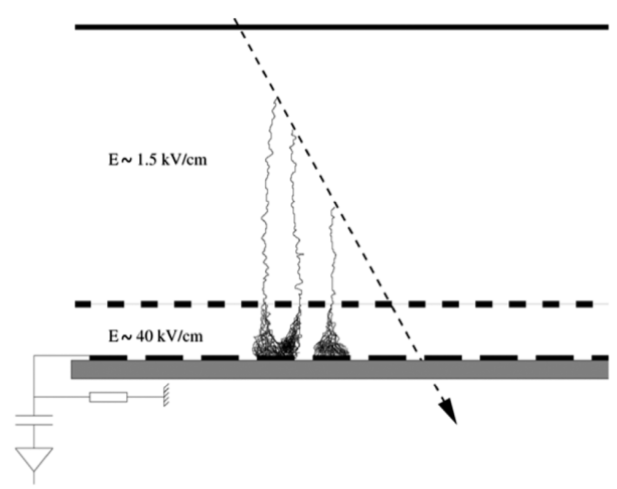
\includegraphics[width=0.6\textwidth]{Figures/Micromegas}
\caption[Principio de funcionamiento de un detector Micromegas]{Principio de funcionamiento de un detector Micromegas \cite{Procureur2018}. Los Micromegas se caracterizan por tener una rejilla interna cuya  función es amplificar la avalancha de electrones y, a su vez, acelerarla con el fin de disminuir el tiempo de respuesta del detector. En este caso, la rejilla genera un campo eléctrico de 40 kV/cm.}
\label{RPC}
\end{center}
\end{figure}

Este tipo de detectores poseen una alta resolución espacial ($\sim 0.1 mm$) a un costo razonable. Además, éstos permiten hacer una trazabilidad temporal de los eventos.\\

Sin embargo, los detectores gaseosos tienen varias desventajas. La ganancia depende altamente de variables ambientales como la presión y la temperatura. El alto voltaje de polarización necesario para su funcionamiento óptimo implica un riesgo latente de generación de chispas eléctricas que afectarían su integridad.  El gas ionizante debe fluir continuamente en el interior del detector con el fin de evitar el envejecimiento y degradación de los electrodos. Finalmente, las fugas de gas son inherentes e inevitables  elevando el costo del mantenimiento del detector.\\

En la Tabla \ref{tab1} se muestra una comparación de las principales características de los hodoscopios dependiendo de la tecnología de detección empleada.  \\

En este caso, los centelladores segmentados ofrecen la mejor alternativa de diseño debido a su bajo consumo energético, simplicidad y gran robustez mecánica, en comparación con las otras tecnologías. Todas estas ventajas se ven reflejadas en la disminución del tiempo de construcción del hodoscopio así como en la confiabilidad de su funcionamiento.\\

\begin{table}[ht]
\centering
  \caption{Comparación de las principales características de detección para hodoscopios basados en diferentes tecnologías.}
  \begin{tabular}{ | c | c | c |  c | c |  c | c |}
    \hline
   & \textbf{R. espacial} & \textbf{Voltaje} & \textbf{ToF}  & \textbf{Complejidad} & \textbf{Robustez**} & \textbf{Costo} \\ \hline
    \textbf{C. continuo*}   & baja  & $<$ 80 V &si  & baja  & alta  & bajo \\ \hline
    \textbf{C. segmentado*} & media & $<$ 80 V &si   & media & alta  & medio \\ \hline
    \textbf{RPCs}            & media & $>$ 8.5 kV &si   & alta  & baja &  alto \\ \hline
    \textbf{MWPCs}            & alta  & $>$ 1 kV &si   & alta  & media & alto \\ \hline
    \textbf{MicroMegas}      & alta  & $>$ 400 V &si   & alta  & media & alto \\ \hline
    \textbf{Emulsión}        & alta  & 0 & no   & baja  & baja  & bajo \\
    \hline
  \end{tabular}
  \label{tab1}
\end{table}

* Usando un fotomultiplicador de silicio (SiPM) como elemento sensor.\\
** Capacidad de un sistema para mantener un funcionamiento aceptable frente a situaciones imprevistas.\\


Finalmente, los hodoscopios utilizados para hacer muongrafía en estructuras volcánicas deben soportar diferentes condiciones meteorológicas, en el sitio de observación, sin ser afectados ni necesitar de un mantenimiento constante.

%####################### Fuentes Ruido ###########

\section{Fuentes de ruido en muongrafía}
La muongrafía es contaminada normalmente por tres fuentes de ruido: los muones de baja energía que son dispersados por la superficie de la estructura escaneada, los muones que ingresan por la parte posterior del detector (muones de albedo) y las partículas generadas por EAS entre el detector y el objeto estudiado.

\subsection{Dispersión de muones de baja energía}

La mayor parte del ruido que contamina la técnica de muongrafía ocurre por los muones de baja energía debido a la dispersión múltiple de Coulomb, \cite{Nishiyama2014,Gomez2017}. En este caso, la dirección del muón incidente en el detector no es la misma que su dirección original, Fig. \ref{Scattering}. La variación del ángulo de incidencia del muón $\Delta \theta = \theta_{fin}-\theta_{ini}$ ocurre por su interacción con los núcleos de los átomos que componen el objeto escaneado \cite{Furlan2013, Pesente2009}.

\begin{figure}[h!]
\begin{center}
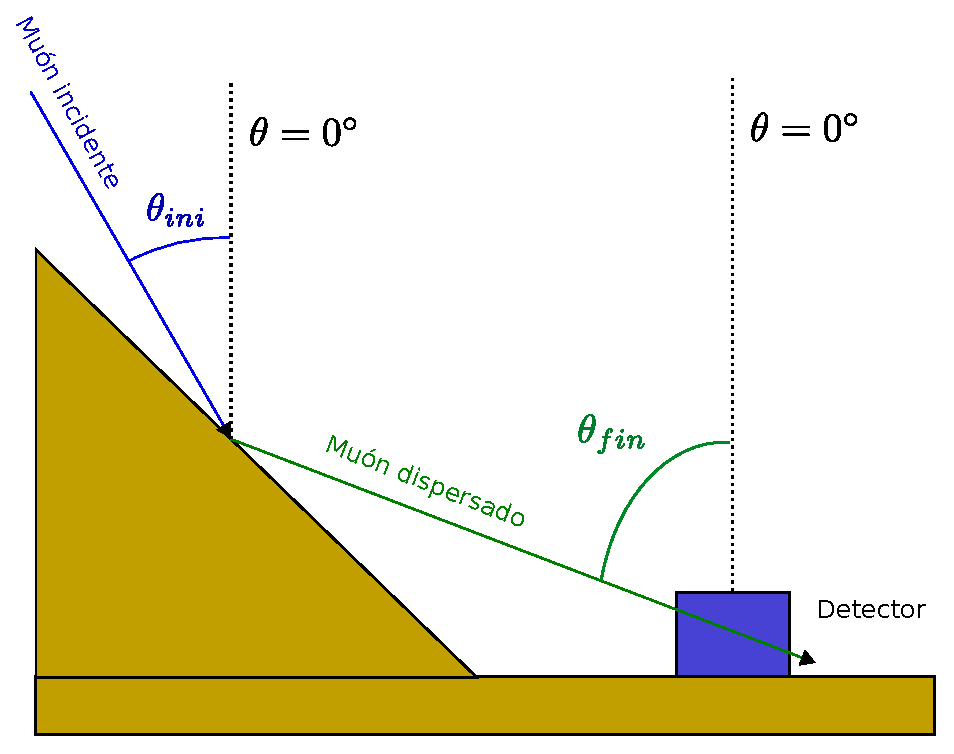
\includegraphics[width=0.65\textwidth]{Figures/Muon_scattering.eps}
\caption[Dispersión de los muones incidentes de baja energía sobre la superficie]{Dispersión de los muones incidentes de baja energía sobre la superficie. El ángulo de incidencia del muón $\theta_{ini}$ varía debido a su interacción con el material que compone la estructura resultando en un ángulo dispersado $\theta_{fin}$. Adaptado de \cite{Gomez2017}.}
\label{Scattering}
\end{center}
\end{figure}


\begin{figure}[h!]
\begin{center}
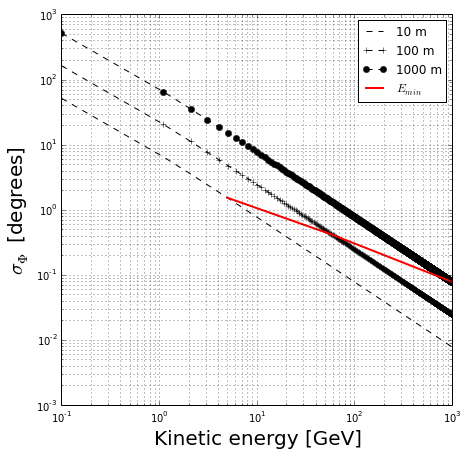
\includegraphics[width=0.6\textwidth]{Figures/Scattering}
\caption[Variación angular, respecto a su dirección de incidencia, de los muones atmosféricos después de atravesar 10 m, 100 m y 1000 m de roca estándar]{Variación angular, respecto a su dirección de incidencia, de los muones atmosféricos después de atravesar 10 m, 100 m y 1000 m de roca estándar. La línea roja representa el umbral de energía mínima sobre el cual los muones logran emerger del medio sin ser absorbidos.}
\label{Scattering_Variance}
\end{center}
\end{figure}

Para evaluar los efectos de la dispersión en los muones incidentes se debe tener en cuenta la energía mínima requerida para atravesar el material, tal como se puede apreciar en la  Fig. \ref{Scattering_Variance}.\\

La dispersión múltiple de Coulomb se puede representar como una distribución Gausiana con media cero y con una desviación estándar $\sigma_\theta$ que depende de la longitud de radiación $X_0$, del espesor del material $x$, de la cantidad de movimiento $p$ y velocidad $\beta$ del muón  \cite{Grupen2008}:

\begin{equation}
\sigma_\theta \approx \frac{13.6 \text{MeV}}{\beta p c} \sqrt{\frac{x}{X_0}}
\end{equation}

\begin{equation}
X_0 = \frac{716.4 (\text{g/cm}^2)}{\rho} \frac{A}{Z(Z+1)\ln (287/\sqrt{Z})}
\end{equation}
donde $\rho$ es la densidad y $Z$ es el número atómico efectivo del material atravesado.


\subsection{Muones de albedo}

Otro factor que repercute en la contaminación de la muongrafía son los muones cuasi-horizontales ($\theta >= 75^{\circ}$) que inciden en el detector desde la parte posterior. El momento promedio de los también llamados muones de albedo es de $\approx 10 GeV/c$ \cite{Nishiyama2014}. Estas partículas trazan trayectorias similares a los muones emergentes desde el volcán generando eventos de coincidencia en el detector. Ver Fig. \ref{Albedo}.

\begin{figure}[h!]
\begin{center}
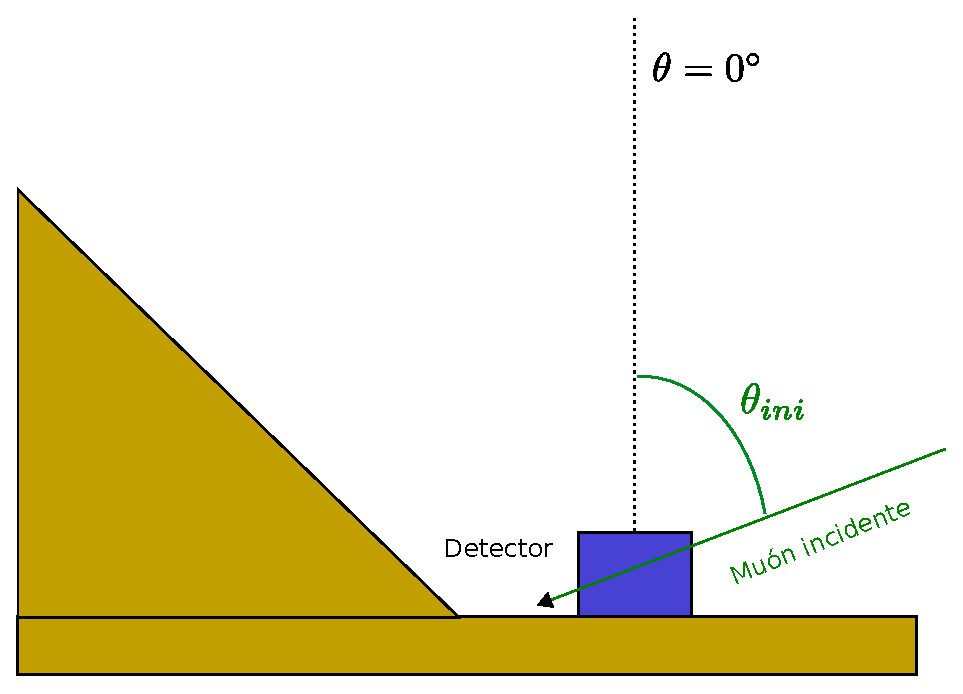
\includegraphics[width=0.65\textwidth]{Figures/Albedo.eps}
\caption[Detección de un evento falso debido a un muón que incide por la parte posterior del detector]{Detección de un evento falso debido a un muón que incide por la parte posterior del detector. La partícula atraviesa el hodoscopio emulando una trayectoria válida proveniente desde la estructura escaneada con un ángulo 180$^\circ$ - $\theta_{ini}$.}
\label{Albedo}
\end{center}
\end{figure}

El espectro de muones a nivel del mar $\Phi(p,\theta,h=0m)$ como función del momento $p$ y el ángulo cenital $\theta$ es dado por \cite{Reyna2006}:


\begin{align*}
\Phi(p,\theta,0) &= \cos^3\theta\Phi_V(p \cos \theta),\\
\Phi_V(\zeta) &= c_1 \zeta^{-(c_2+c_3\log_{10}\zeta+c_4(\log_{10}\zeta)^2+c_5(\log_{10}\zeta)^3)},\\
c_1 &= \text{0.00253cm}^{-2}s^{-1}sr^{-1}(GeV/c^{-1}),\\
c_2 &= \text{0.2455},c_3=\text{1.288},c_4=\text{-0.2555},c_5=\text{0.0209}
\end{align*}

donde $\zeta=p\cos\theta$.

\begin{figure}[h!]
\begin{center}
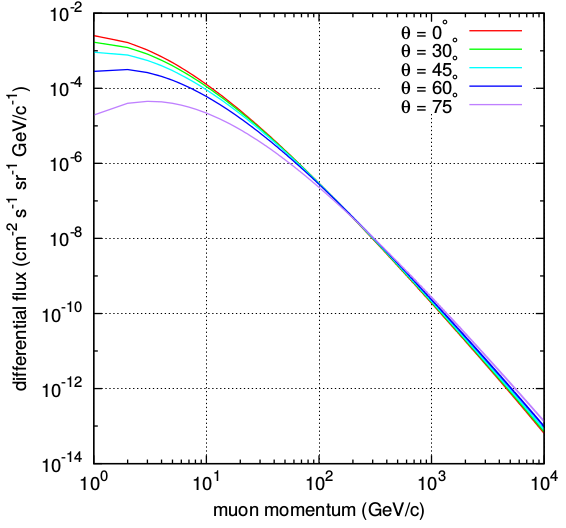
\includegraphics[width=0.65\textwidth]{Figures/Muon_spectrum.png}
\caption[Espectro de energía de muones atmosféricos a diferentes ángulos cenitales]{Espectro de energía de muones atmosféricos a diferentes ángulos cenitales \cite{Ariga2018, Vesga2018, Valencia2016}. El flujo diferencial de muones disminuye a medida que aumenta el ángulo cenital, teniendo una atenuación hasta de dos órdenes de magnitud a 75$^\circ$ (violeta) en comparación con el flujo a 0$^\circ$ (rojo).}
\label{Muon_spectrum}
\end{center}
\end{figure}

Como se puede ver en la Fig. \ref{Muon_spectrum} el flujo de muones a nivel del mar disminuye a medida que el ángulo cenital aumenta. Por otro lado, el momento promedio aumenta con el incremento del cenit teniendo de esta manera que el momento promedio para los muones verticales es de $\approx$ 4 GeV/c y de los quasi-horizontales es de $\approx$ 10 GeV/c.\\

Esta fuente de ruido puede ser significativa si el detector se encuentra ubicado en un sitio en el cual no tenga ninguna clase de protección en su parte posterior, por ejemplo, cadenas montañosas que sirvan como filtro a estos muones quasi-horizontales.

\subsection{Componente electromagnética (EM) de EAS}

La tercera fuente de contaminación en la muongrafía ocurre debido a partículas secundarias (PS) generadas por EAS entre la estructura escaneada y el detector. Ver Fig. \ref{EAS}.\\

Las PS están compuestas principalmente por $p,n,\mu^{\pm},\pi^{\pm},e^{\pm}$ y $\gamma$. El flujo de PS como función de la energía cinética es presentado en la Fig. \ref{Particle_Flux}. El flujo de PS a nivel del mar es estimado, por medio de una simulación, teniendo en cuenta el espectro de rayos cósmicos primarios que inciden sobre la atmósfera terrestre. En la simulación la componente  electromagnética es cortada bajo 1 MeV para $e^{\pm}$ y bajo 100 keV para $\gamma$.

\begin{figure}[h!]
\begin{center}
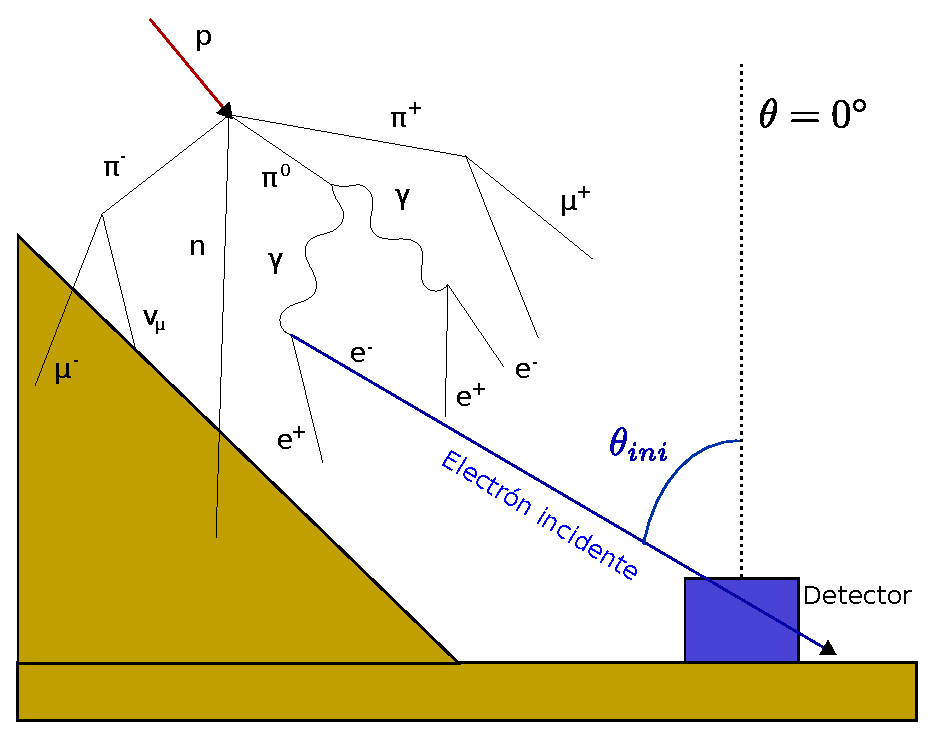
\includegraphics[width=0.65\textwidth]{Figures/EAS.eps}
\caption[Detección de un evento falso debido a la incidencia de un $e^-$ generado en una EAS entre el objeto escaneado y el detector]{Detección de un evento falso debido a la incidencia de un $e^-$ generado en una EAS entre el objeto escaneado y el detector. Las partículas cargadas de la componente EM de las EAS generan un aumento en el flujo estimado al atravesar el hodoscopio.}
\label{EAS}
\end{center}
\end{figure}

Las partículas más abundantes son los $\gamma$ seguidos por los $n$ y $\mu^{\pm}$. Los $e^{\pm}$ y $p$ tienen flujos menores y los $\pi^{\pm}$ son tres órdenes de magnitud menos probables.\\

\begin{figure}[h!]
\begin{center}
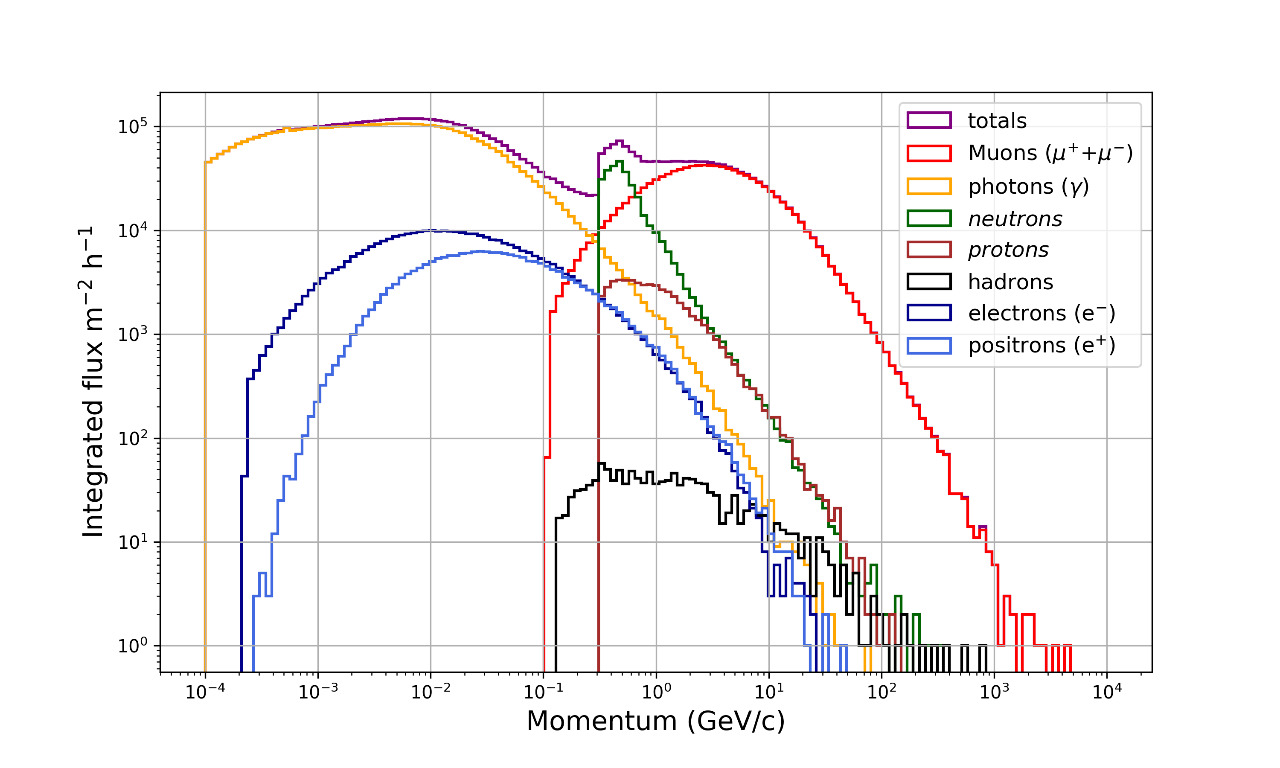
\includegraphics[width=1\textwidth]{Figures/PS_Flux}
\caption[Flujo de PS simulado a nivel del volcán Cerro Machín]{Flujo de PS simulado a nivel del volcán Cerro Machín para el Telescopio de Muones (MuTe) en Colombia, \cite{Vasquez2018, Valencia2016}. El espectro esta compuesto por los flujos individuales de $p,n,\mu^{\pm},\pi^{\pm},e^{\pm}$ y $\gamma$. En este caso, predominan dos jorobas, una centrada en $\sim 10$ MeV/c compuesta por $e^{\pm}$ y $\gamma$ y otra a $\sim 3$ GeV/c compuesta por $\mu^{\pm}$.}
\label{Particle_Flux}
\end{center}
\end{figure}

La estructura general del espectro de PS a nivel de suelo tiene dos jorobas predominantes que se solapan alrededor de 0.3 GeV/c. La primera joroba representa la componente electromagnética de la EAS y está compuesta principalmente por $e^{\pm}$ y $\gamma$. Por otro lado, la segunda joroba representa la componente muónica conformada por $\mu^{\pm}$.\\

Las PS generan eventos falsos de dos maneras:

\begin{itemize}
    \item Mediante la coincidencia accidental de dos o más partículas incidentes en el detector lo cual mimetiza una trayectoria generada por un muón \cite{KUSAGAYA2015}.
    \item Una partícula individual con energía suficiente para atravesar todo el detector.
\end{itemize}

Teniendo en cuenta que la muongrafía hace una estimación de la distribución densidad interna de la estructura dependiendo del flujo diferencial de los muones que la atraviesan, un aumento en el flujo registrado debido a los eventos falsos repercute en una sub-estimación de la densidad de la estructura, \cite{Nishiyama2014}.

%############# Eliminación de Ruido #######################

\section{Eliminación de ruido en muongrafía}

La discriminación de eventos falsos en muongrafía presenta un reto actual. Este proceso se puede efectuar mediante la medición de las características diferenciadoras entre las partículas que generan señal y las que generan ruido.\\

En este contexto, las técnicas de identificación de partículas (PID) surgen como solución en la tarea de discriminación \cite{Nishiyama2016}. Las técnicas PID se basan principalmente en la medición de 4 variables: el tiempo de vuelo (ToF), la pérdida de energía, la radiación Cherenkov (contadores, RICH y DISC) y la radiación de transición. En la Fig. \ref{PID} se muestra una comparación de los métodos PID y su rango de operación.

\begin{figure}[h!]
\begin{center}
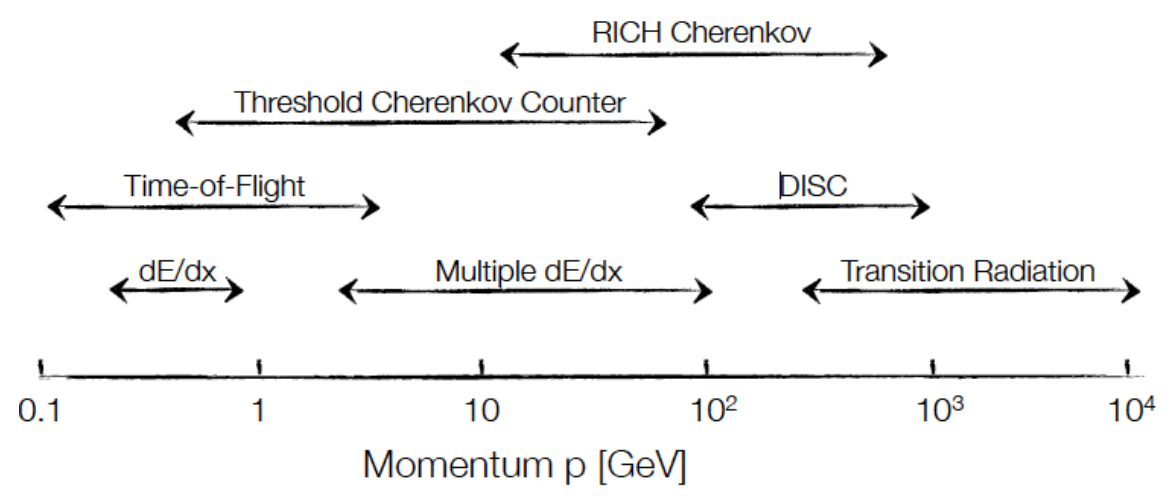
\includegraphics[width=0.8\textwidth]{Figures/PID}
\caption[]{Comparación de métodos PID para diferenciar $\pi^{\pm}$ y $K^{\pm}$ \cite{Kleinknecht2005}}
\label{PID}
\end{center}
\end{figure}

Las principales componentes del ruido de fondo en muografía son muones y electrones de baja energía ($<$ 1 GeV), por lo cual pueden ser identificadas mediante la medición de la pérdida de energía, los contadores Cherenkov o sistemas ToF.

\subsection{Medición del tiempo de vuelo}

La medición del ToF de la partícula permite estimar su velocidad, su momento \cite{Best2015} y su identidad \cite{Gruttola2014, Kolanoski2016}. Adicionalmente, la medición del momento en muongrafía puede ser usada para filtrar las partículas con momento $<$ 1 GeV/c las cuales componen la principal fuente de ruido en esta técnica como se reporta en \cite{Nishiyama2014,Gomez2017}.

En la Fig. \ref{ToF} (línea sólida) se muestra el ToF  para muones con momento entre 0.1 GeV/c y 100 GeV/c medido por un hodoscopio de dos paneles centelladores con una separación de 1 m. A medida que el cantidad de movimiento aumenta el ToF decrece hasta que llega a una zona de saturación debido a los límites relativistas para momentos $>$ 1 GeV/c, en esta región el ToF es $\approx 3.3 ns$.

\begin{figure}[h!]
\begin{center}
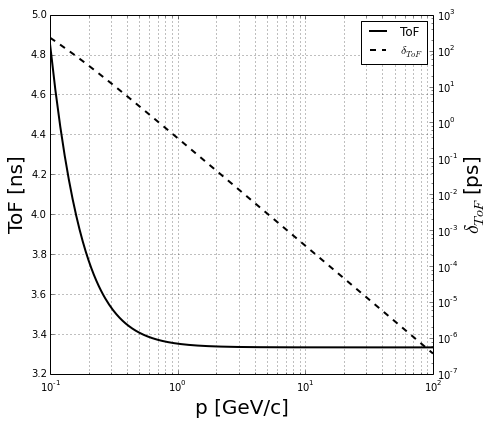
\includegraphics[width=0.55\textwidth]{Figures/ToF_Mix.png}
\caption[Resolución del ToF necesaria para diferenciar muones con momento entre 0.1 GeV/c y 100 GeV/c con un $\sigma_p = 10$ MeV]{(Línea sólida): Tiempo de vuelo para muones con momento entre 0.1 GeV/c y 100 GeV/c al atravesar un hodoscopio de dos paneles con 1 m de separación \cite{Williams2012, Best2015}. (Línea punteada): Resolución del ToF necesaria para diferenciar muones con momento entre 0.1 GeV/c y 100 GeV/c con un $\sigma_p = 10$ MeV al atravesar un hodoscopio de dos paneles con 1 m de separación \cite{Genat2009, Lippmann2012}.}
\label{ToF}
\end{center}
\end{figure}

% \begin{figure}[h!]
% \begin{center}
% 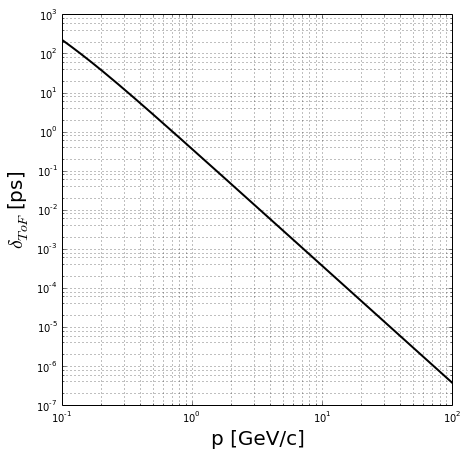
\includegraphics[width=0.55\textwidth]{Figures/ToF_Resolution.png}
% \caption[Resolución del ToF necesaria para diferenciar muones con momento entre 0.1 GeV/c y 100 GeV/c con un $\sigma_p = 10$ MeV]{Resolución del ToF necesaria para diferenciar muones con momento entre 0.1 GeV/c y 100 GeV/c con un $\sigma_p = 10$ MeV al atravesar un hodoscopio de dos paneles con 1 m de separación \cite{Genat2009, Lippmann2012}.}
% \label{Resolution}
% \end{center}
% \end{figure}

La resolución del momentum del detector mide su habilidad para distinguir partículas con momentos cercanos. En este caso, la resolución de la cantidad de movimiento depende de la resolución del ToF. Para el hodoscopio anteriormente expuesto la resolución del ToF para muones con momentos entre de 0.1 GeV/c y 100 GeV/c se expone en la Fig. \ref{ToF} (línea punteada). Por ejemplo, para medir un momento de 1 GeV/c con una $\sigma_p = 10$ MeV es necesario un $\delta_{ToF}\approx$ 1 ps y para 10 GeV/c un $\delta_{ToF}\approx$ 0.003 ps.\\

%Adicionalmente, el ToF es también usado para identificación de partículas \cite{Kolanoski2016}. En este caso, ofrecería una herramienta para diferenciar los $e^{\pm}$ provenientes de EAS de los $\mu^{\pm}$ emergentes desde el volcán.\\

En la Fig. \ref{ToF_mue} se muestra el ToF registrado en un hodoscopio, con 1 m de separación entre sus planos, para $\mu^{\pm}$ y $e^{\pm}$ a nivel del mar teniendo en cuenta su espectro de la Fig. \ref{Particle_Flux}. En este caso, el proceso de discriminación es viable para momentos $\le 10$ MeV/c para $e^{\pm}$ y $\le 2$ GeV/c para $\mu^{\pm}$ , por encima de estos valores estas partículas describen el mismo ToF. \\

El ToF permite además discriminar los muones de albedo debido a que muestran un ToF negativo ya que inciden primero en el panel posterior del hodoscopio.

\begin{figure}[h!]
\begin{center}
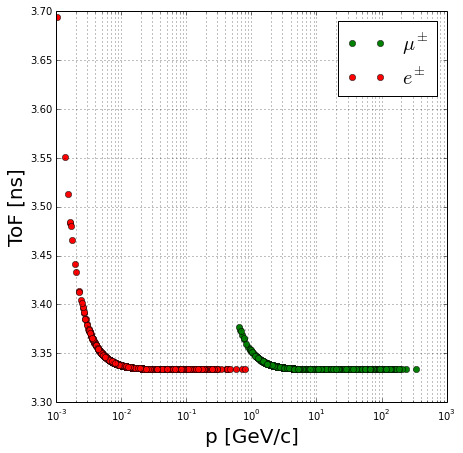
\includegraphics[width=0.5\textwidth]{Figures/ToF_Spec.png}
\caption{Tiempo de vuelo para $\mu^{\pm}$ (verde) y $e^{\pm}$ (rojo) al atravesar un hodoscopio de dos paneles con 1 m de separación. El límite de discriminación de $\mu^{\pm}$ es $\sim$ 2 GeV y para $e^{\pm}$ de $\sim$ 10 MeV}
\label{ToF_mue}
\end{center}
\end{figure}
 
\subsection{Medición de la pérdida de energía}

La estimación de la -dE/dx se hace por medio de un calorímetro el cual puede ser continuo o segmentado. Este dispositivo mide la cantidad de luz generada por la partícula incidente al ionizar el medio que cruza.\\

Los contadores Cherenkov miden los fotones generados por una partícula cargada al cruzarlo. En este caso, cuando la velocidad de la partícula es mayor a la velocidad de la luz en el medio, el medio sufre un proceso de polarización-depolarización que genera una onda electromagnética plana por interferencia constructiva \cite{Kolanoski2016}.\\

El ángulo de emisión de los fotones Cherenkov $\theta_c$ es definido como:

\begin{equation}
    \cos \theta_c = \frac{1}{n\beta}
\end{equation}
donde $n$ es el índice de refracción del medio.

\begin{figure}[h!]
\begin{center}
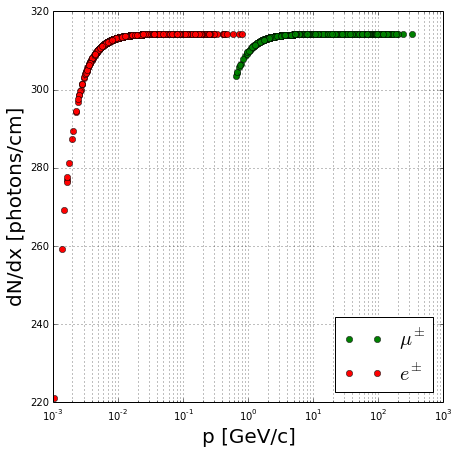
\includegraphics[width=0.5\textwidth]{Figures/dNdx_spec.png}
\caption[Fotones Cherenkov por unidad de longitud generados por $\mu^{\pm}$ y $e^{\pm}$ a nivel del mar en el rango de 300nm $< \lambda <$ 570nm]{Fotones Cherenkov por unidad de longitud generados por $\mu^{\pm}$ y $e^{\pm}$ a nivel del mar en el rango de 300nm $< \lambda <$ 570nm\cite{Vasquez2018, Motta2018}.}
\label{dNdx}
\end{center}
\end{figure}

Así mismo, el número de fotones Cherenkov por unidad de longitud es:

\begin{equation}
   \frac{dN}{dx}=2 \pi \alpha z^2 \int_{\lambda_1}^{\lambda_2} \left(1- \frac{1}{n^2 \lambda \beta^2} \right) \frac{d \lambda}{\lambda^2} \approx 2 \pi \alpha z^2 \sin^2 \theta_c \left( \frac{\lambda_2-\lambda_1}{\lambda_2 \lambda_1} \right) 
\end{equation}

donde $\alpha$ es la constante de estructura fina, $z$ representa la carga de la partícula en unidades de la carga del electrón $e$ y $\lambda$ es la longitud de onda de la radiación Cherenkov.\\ 

Por ejemplo, para un rango de longitudes de onda que incluye el espectro visible y ultravioleta ($\lambda_1 =$ 300 nm - $\lambda_2 =$ 570 nm) tenemos:

\begin{equation}
   \frac{dN}{dx} \approx 723 \sin^2 \theta_c \ \text{[photons/cm]}
\end{equation}

%La medición de la pérdida de energía (-dE/dx) permite la identificación de partículas \cite{Klinger2015}.

En la Fig. \ref{dNdx} se muestra el número de fotones Cherenkov (dN/dx) por centímetro que generan los $e^{\pm}$ y $\mu^{\pm}$ en un contador Cherenkov de agua. En este caso, la dN/dx para $e^{\pm} > $  10 MeV/c y para $\mu^{\pm} > $ 2 GeV/c es de $\approx 315$ fotones/cm. 

\begin{figure}[h!]
\begin{center}
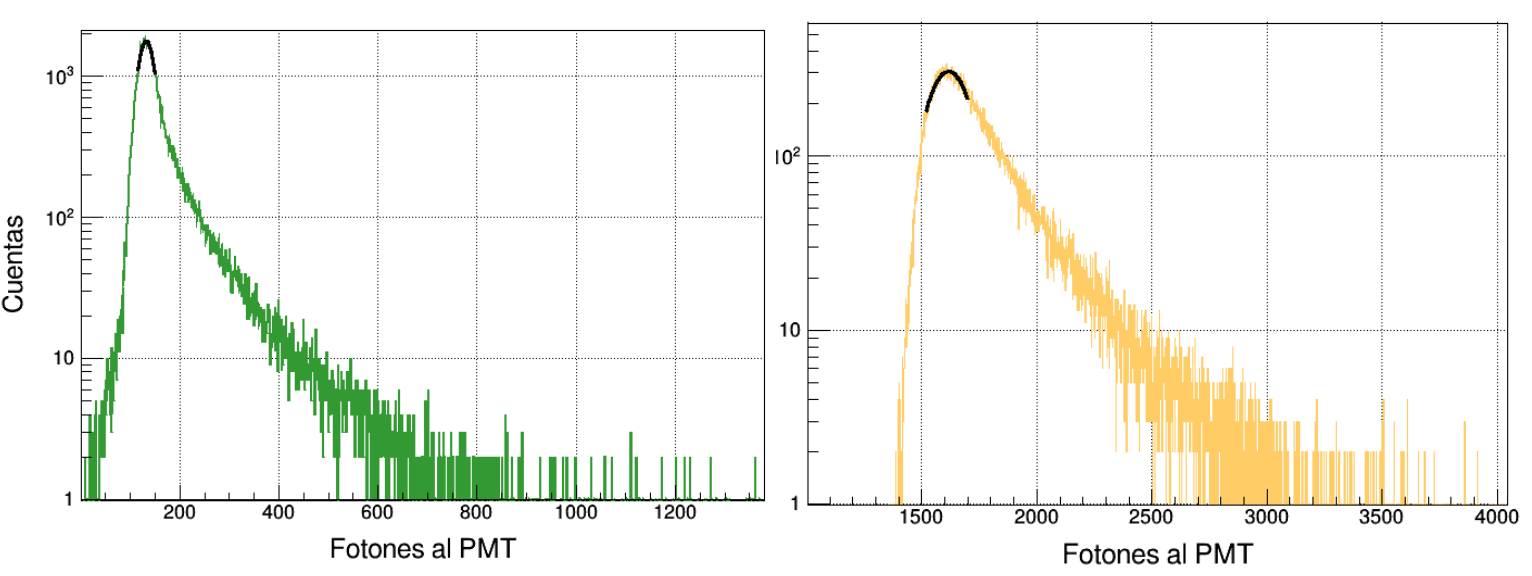
\includegraphics[width=1\textwidth]{Figures/e_mu_hist.png}
\caption[Histograma del número total de fotones Cherenkov generados por $1\times10^5$ $e^-$ de 20 MeV y $1\times10^5$ $\mu^-$ de 3 GeV en un contador Cherenkov de agua]{Histograma del número total de fotones Cherenkov generados por $1\times10^5$ $e^-$ de 20 MeV y $1\times10^5$ $\mu^-$ de 3 GeV en un contador Cherenkov de agua \cite{Vasquez2018}.}
\label{N_mue}
\end{center}
\end{figure}

No obstante, los $e^{\pm}$ son frenados rápidamente por el medio debido a su pérdida de energía generando un número total de fotones $N$ menor al causado por los $\mu^{\pm}$ los cuales recorren una distancia mayor. En la Fig. \ref{N_mue} se muestran los histogramas del número de fotones que alcanzan el dispositivo sensor (PMT) en un detector Cherenkov cúbico de agua con 1.2 m de lado. \\

Debido a que los $e^{\pm}$ pueden recorrer una longitud promedio de 10 cm siendo $N \approx 200$, en contraste, los $\mu^{\pm}$ atraviesan totalmente el contador Cherenkov generando $N \approx 1600$. Teniendo en cuenta esto, la medición de la radiación Cherenkov permite separar la componente electromagnética y la componente muónica de las EAS.

\chapter{Metodología}

A continuación se describe detalladamente la metodología que se ha llevado a cabo para el cumplimiento de los objetivos del proyecto de investigación. En cada actividad también se describen los resultados preliminares obtenidos.

\section{Diseño y calibración del sistema electrónico del hodoscopio}

Para la medición del flujo de partículas dependiendo de la trayectoria se desarrollará un hodoscopio con dos paneles compuestos de 60 centelladores plásticos cada uno. Cada centellador tendrá un SiPM S13360-6050CS como elemento sensor. Las señales de cada panel serán discriminadas mediante un sistemas de adquisición (DAQ) basado en el Circuito de Aplicación Específica (ASIC) MAROC3A para luego ser almacenadas. El sistema DAQ es controlado por un computador embebido Rapsberry Pi. El hodoscopio tendrá un sistema de disparo estratificado que determinará la veracidad de los eventos detectados y las coincidencias entre los paneles que lo conforman. \\

Por otro lado, los SiPM serán caracterizados con el fin de determinar su comportamiento (ganancia y ruido) dependiendo de la temperatura y el voltaje de ruptura. La atenuación de la señal en las barras centelladoras será medida para diferentes puntos de interacción usando un sistema de estimulación controlado. Adicionalmente, se evaluará la respuesta de los paneles centelladores y el hodoscopio midiendo el flujo de muones atmosféricos en diferentes direcciones. Los resultados preliminares y detalles técnicos de las actividades relacionadas con este objetivo se muestran a continuación.\\


\textbf{Actividades y resultados preliminares}\\

\subsection{Diseño del hodoscopio}

El hodoscopio está formado por dos paneles sensibles compuestos de $30 \times 30$ barras centelladoras rectangulares de $120 \textrm{cm} \times 4 \textrm{cm} \times 1 \textrm{cm}$.\\

Los centelladores, fabricados por Fermilab, están hechos de poliestireno (Dow Styron $663$) con un recubrimiento externo de TiO$_2$ de 0.25 mm de espesor. Los dopantes del material primario son $1\%$ PPO  y $0.03 \%$ POPOP, con un pico máximo de emisión en 420 nm \cite{Anghel2015} y un tiempo de decaimiento de 1.6 ns \cite{Kleinknecht2005}. \\

Cada barra centelladora tiene un agujero de 1.8 mm de diámetro en su parte central donde va situada una fibra óptica de corrimiento de longitud de onda (WLS). En este caso se usa la fibra Saint-Gobain BCF-92 con un diámetro de 1.2 mm, un índice de refracción en el núcleo de 1.42, un pico de absorción de 410 nm y un pico de emisión de 492 nm \cite{Kuraray2018}.\\

En este caso se usa el SiPM Hamamatsu S13360-6050CS como elemento sensor. El SiPM tiene un área fotosensible de 
$1.3 \times 1.3 \textrm{mm}^2$, 667 píxeles, un factor de llenado 74$\%$, un voltaje de ruptura de 53$\pm$5 V (25 $^{\circ}$C), una ganancia de $10^5$ a $10^6$ y una eficiencia de foto-detección de  40$\%$ a 450 nm.\\

Los SiPM están acoplados de manera directa con la fibra óptica mediante un sistema mecánico anclado a la barra centelladora. Este sistema centra el extremo de la fibra óptica con la región sensible del SiPM. Ver Fig. \ref{SiPM_WLS}. Usualmente se utiliza resina óptica EJ200 de Eljen Technology para acoplar el SiPM y la fibra óptica, sin embargo, resultados de la simulación del centellador-fibra-SiPM en GEANT4 \cite{Vasquez2018} demuestran que su uso no aumenta el número de fotones que llegan al SiPM.

\begin{figure}[h!]
\begin{center}
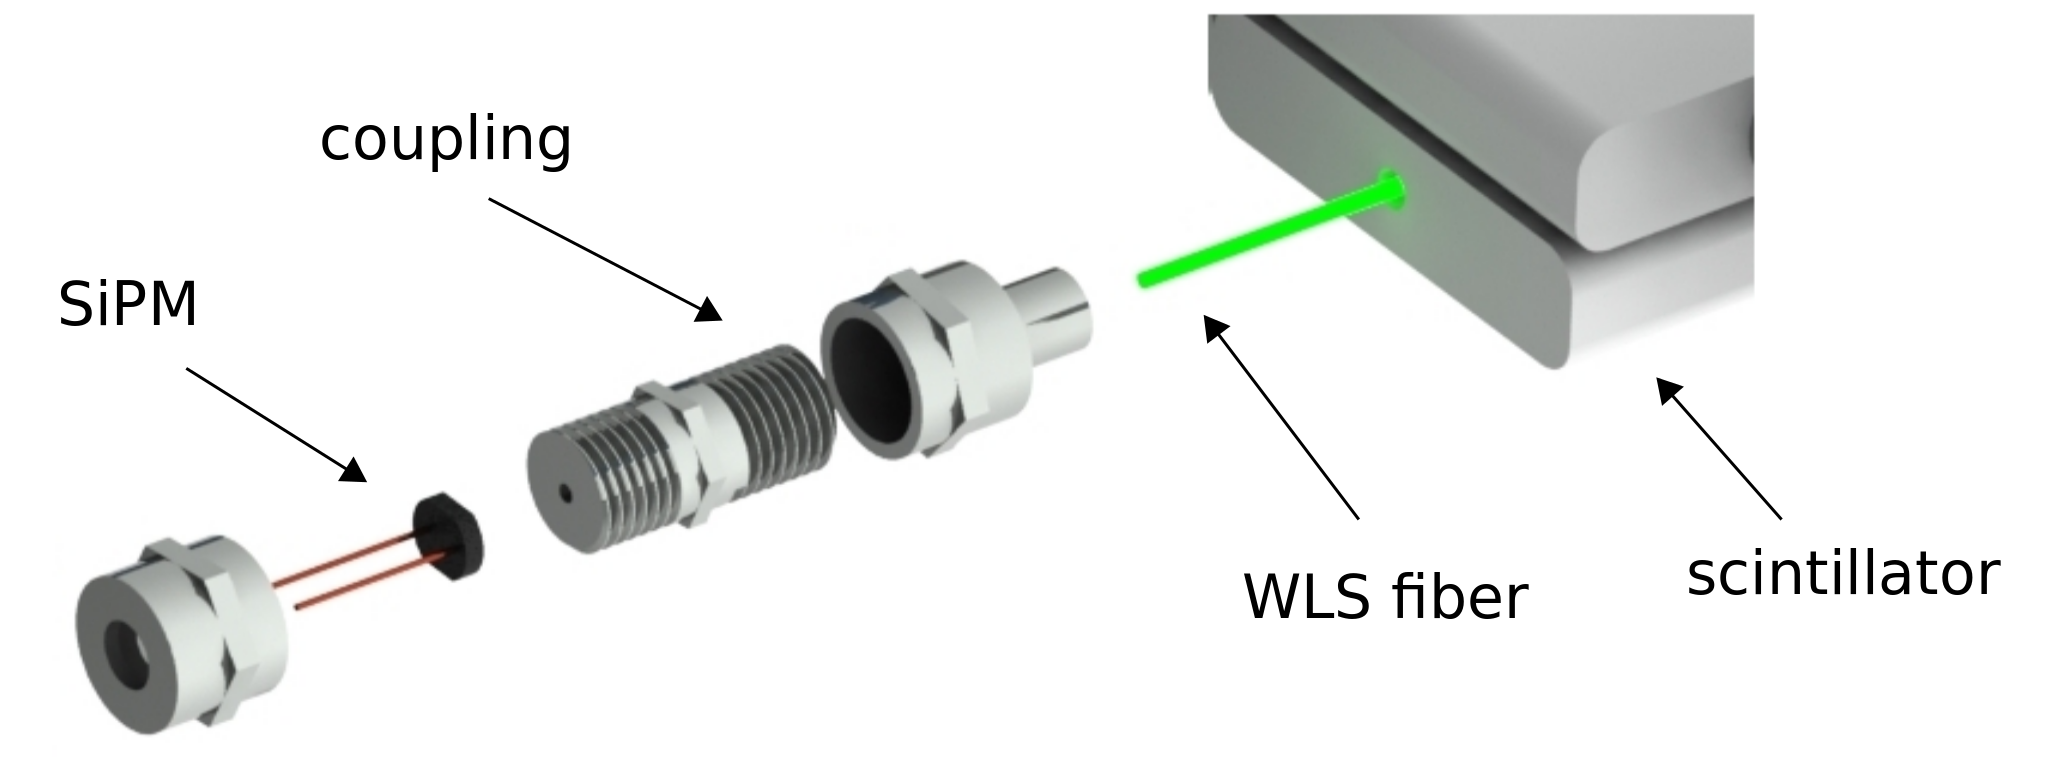
\includegraphics[width=0.7\textwidth]{Figures/panel_frontend.png}
\caption{Sistema de acople entre la fibra WLS y el SiPM en cada barra centelladora.}
\label{SiPM_WLS}
\end{center}
\end{figure}

\subsection{Diseño de la electrónica del SiPM}

 La electrónica de acondicionamiento consta de una etapa de polarización del SiPM, una etapa de amplificación (con ganancia 94) y un acople de impedancias como se muestra en Fig. \ref{SiPM_Ele}. 
 
 El circuito de polarización alimenta el SiPM con un voltaje (HV) que varia entre 40V y 80V. La fuente HV se basa en el módulo controlable C11204 de Hamamatsu.
 
 \begin{figure}[h!]
\begin{center}
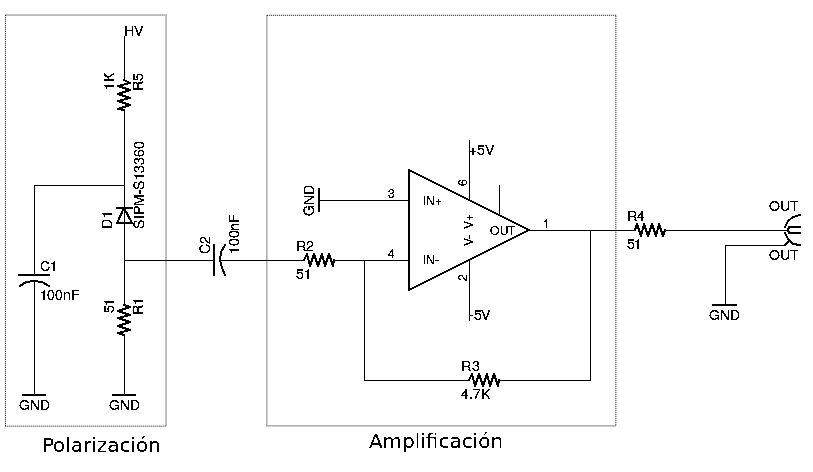
\includegraphics[width=0.7\textwidth]{Figures/Acondicionamiento.png}
\caption{Electrónica de polarización y acondicionamiento del SiPM.}
\label{SiPM_Ele}
\end{center}
\end{figure}

La fuente HV se basa en el módulo controlable C11204 de Hamamatsu el cual puede proporcionar voltajes entre 40V y 80V. Por otra parte, la amplificación de la señal pulsada se hace mediante el amplificador operacional OPA691 de Texas Instruments cuyo ancho de banda es 190 MHz. Finalmente, la señal amplificada se transmite a través de un cable coaxial RG178U con impedancia de 50 ohmnios y ancho de banda de 900 MHz.

\subsection{Diseño del sistema de adquisición del hodoscopio}

El sistema de adquisición se basa en el Circuito Integrado de Aplicación Específica (ASIC) MAROC3A de Omega, desarrollado para aplicaciones en detectores de partículas.

\begin{figure}[h!]
\centering
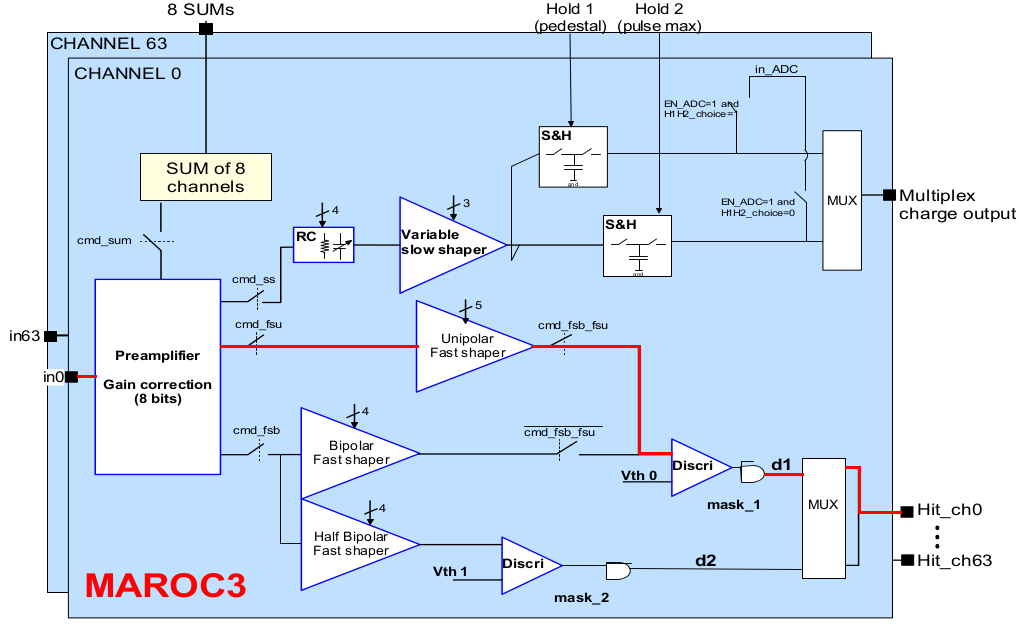
\includegraphics[scale=0.5]{Figures/Maroc.png}
\caption{Architectura del ASIC MAROC3A. La línea roja indica las etapas que recorre cada señal hasta su discriminación.}
\label{Maroc}
\end{figure}


La MAROC3A tiene 64 canales de lectura con una impedancia de entrada de 50 ohmios. Cada canal tiene una etapa de amplificación de ganancia programable (0-4), un \textrm{fast-shaper} unipolar con ganancia de 2.3V/pC y un discriminador (d1) con un umbral de discriminación ($V_{th0}$) establecido por un Convesor Digital-Análogo (DAC) de 10 bits (2.3 mV/UDAC). En la Fig. \ref{Maroc} se muestra el hilo que sigue un canal en la MAROC3A.\\

En este caso se usan solamente 60 de los 64 canales. Las señales son transportadas desde el panel centellador a través de cables coaxiales RG178U con impedancia de 50 ohmios y ancho de banda de 900 MHz. Todos los cables tienen la misma distancia (2.9 m) para evitar diferencias temporales entre canales.\\

Los parámetros de configuración de: la ganancia de amplificación, el umbral de discriminación, la elección de los $shapers$ y los discriminadores, así como la habilitación/des-habilitación de canales se hace a través de una FPGA Cyclone III de Altera. Esta información se transmite a la MAROC3A en una trama de 829 bits.\\

Los datos resultado de proceso de discriminación se ordenan en un vector de 8 bytes (64 bits - 64 canales). Cada bit toma el valor "1" si la señal de dicho canal supera el umbral de discriminación, sino toma el valor "0". Simultáneamente, cuando ocurre un evento en alguno de los 64 canales, se genera una señal de disparo (OR-Trigger o T1).\\

La adquisición de eventos en cada panel es controlada por un computador embebido (Raspberry Pi 2 - SCB) el cual almacena los datos y meta-datos de cada panel. Los datos contienen la información de las barras disparadas, el tiempo de ocurrencia del evento, el ToF, la presión atmosférica, temperatura y consumo eléctrico (I/V).\\

En la Fig. \ref{DAQ} se muestra el diagrama de flujo del sistema de adquisición para un panel de centelleo. La MAROC3A genera una señal de disparo cuando un evento sobrepasa el umbral de discriminación, esta señal de disparo es distribuida (Trigger-split) en tres direcciones: a la MAROC3A (Ext-Trigger), al otro panel (P1-P2-Trigger) y al sistema maestro de disparo (P1-Trigger). El Ext-Trigger indica a la MAROC3A que almacene temporalmente el evento registrado. El maestro de disparo (FPGA Spartan 6) evalúa la coincidencia temporal de los disparos mediante una compuerta AND y mide el ToF entre (P1-Trigger y P2-P1-Trigger). Cuando ocurre un evento en coincidencia se envía una señal de interrupción (Int) al SCB para transmitir los datos desde la MAROC3A y almacenarlos en la memoria de la SCB. Durante el proceso de transmisión se activa la señal (Busy) para evitar el solapamiento de eventos.\\

\begin{figure}[h!]
\centering
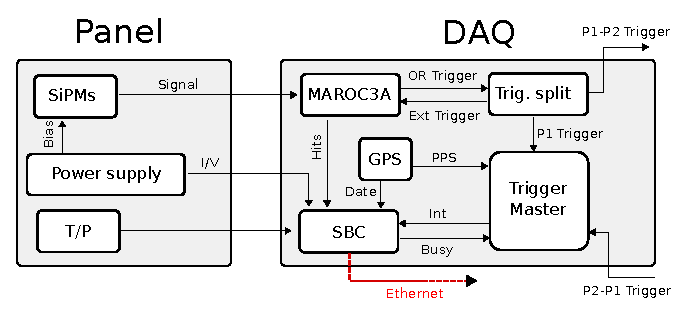
\includegraphics[scale=1.2]{Figures/DAQ.eps}
\caption{Esquema general del sistema de adquisición para un panel centellador.}
\label{DAQ}
\end{figure}

La estampa temporal de los eventos se divide en tres partes: una estampa cada segundo controlada por la señal PPS (Pulse-Per-Second) del GPS, una estampa de 10 ns de resolución establecida por el sistema central de disparo y sincronizada con el PPS y la medición del ToF a una resolución esperada del orden de ps.\\

Los metadatos de temperatura, presión atmosférica y consumo eléctrico se almacenan cada minuto. Finalmente, los datos se almacenan en archivos de una hora de registro cuyo nombre se establece la fecha en el formato Year$\_$ Month$\_$Day$\_$Hour.dat.


\subsection{Caracterización y calibración de los SiPM}

La caracterización del SiPM juega un papel importante ya que permite conocer parámetros como: voltaje de ruptura, , espectro de del foto-electrón, ganancia, conteo oscuro, \textit{cross-talk} y \textit{after-pulse} \cite{sensL2011}. En este caso, se muestra brevemente la metodología de la medición de estos parámetros . 

\subsubsection{Voltaje de ruptura}

El voltaje de ruptura ($V_b$) del SiPM se define como el voltaje de polarización a partir del cual el SiPM funciona en modo Geiger, es decir, el SiPM genera un pulso de corriente cuando un fotón lo impacta. El voltaje de ruptura en el SiPM varia con la temperatura y se determina mediante la curva I-V del SiPM en condiciones de oscuridad.\\

En este caso, las curvas I-V del SiPM se obtuvieron para un rango de temperaturas desde 0$^{\circ}$C hasta 40$^{\circ}$C y una variación del voltaje de polarización de 40V a 60V. Los resultados se muestran en la Fig. \ref{IVSiPM}. Para temperatura ambiente 25$^{\circ}$C, el voltaje de ruptura es 52.3V.

\begin{figure}[h!]
\centering
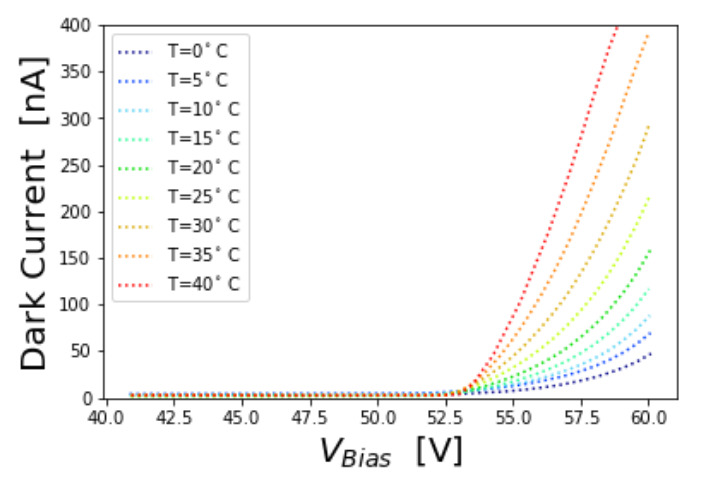
\includegraphics[scale=0.32]{Figures/IVSiPM.jpeg} 
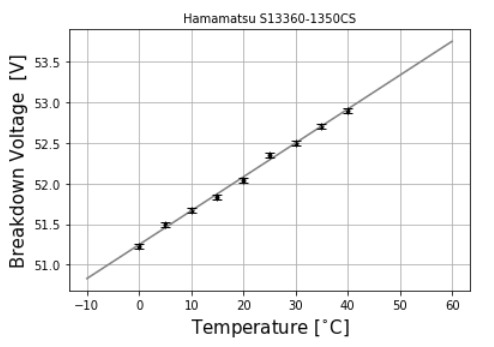
\includegraphics[scale=0.48]{Figures/VbT.jpeg}
\caption{Curvas I-V para el SiPM Hamamatsu 13360-1350CS para temperaturas desde 0$^{\circ}$C hasta 40$^{\circ}$C (izquierda). Dependencia de la temperatura del voltaje de ruptura del SiPM Hamamatsu13360-1350CS (derecha). }
\label{IVSiPM}
\end{figure}

\subsubsection{Espectro de foto-electrón}

El SiPM está formado por una arreglo de foto-diodos de avalancha (APD) conectados en paralelo. La amplitud del pulso de corriente generado es proporcional al número de fotones que inciden sobre él. El espectro de foto-electrón determina el valor equivalente en corriente (o voltaje) de un foto-electrón (p.e.). Este parámetro permite estimar otros parámetros del SiPM como la ganancia, conteo oscuro, \textit{cross-talk} y \textit{after-pulse}.\\

Para obtener dicho espectro, el SiPM fue excitado con una fuente LED pulsada de $\sim$470nm, un ancho de pulso $\sim$9ns, una frecuencia de 500Hz a 25$^{\circ}$C. Los pulsos fueron digitalizados mediante una Red Pitaya con una frecuencia de muestreo de 125 MSPS a 14 bits.\\

Los resultados se exponen el la Fig. \ref{Charge}. El histograma de persistencia se obtuvo con 10000 pulsos. En este caso,  el voltaje de un p.e. estimado es $\sim$13.5mV (izquierda). Por otra parte, el histograma de carga muestra 11 picos de los cuales el primero es el pedestal. La distancia entre picos determina el equivalente en carga de un p.e. $\sim$120ADC.

\begin{figure}[h!]
\centering
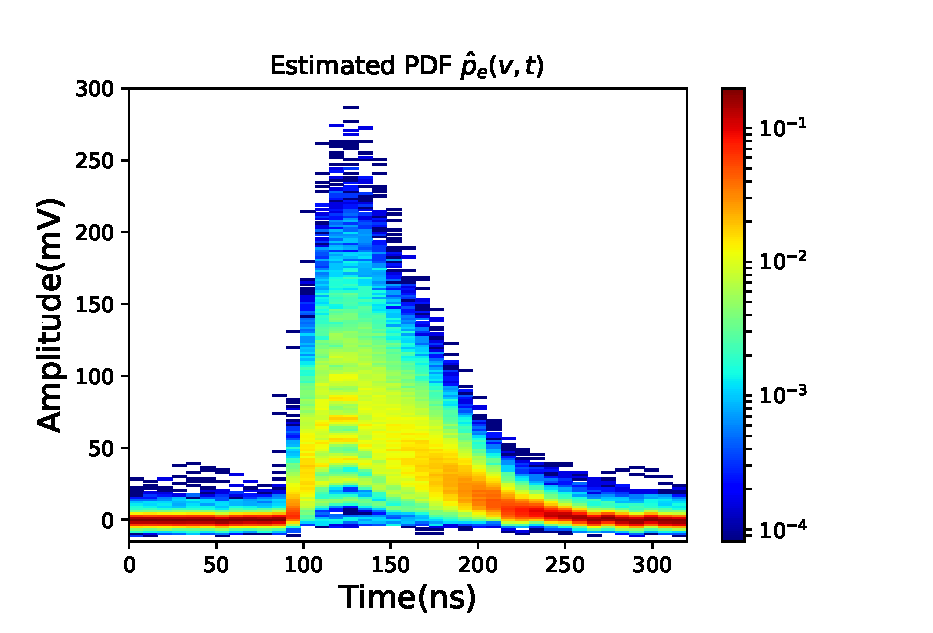
\includegraphics[scale=0.55]{Figures/Pulses} 
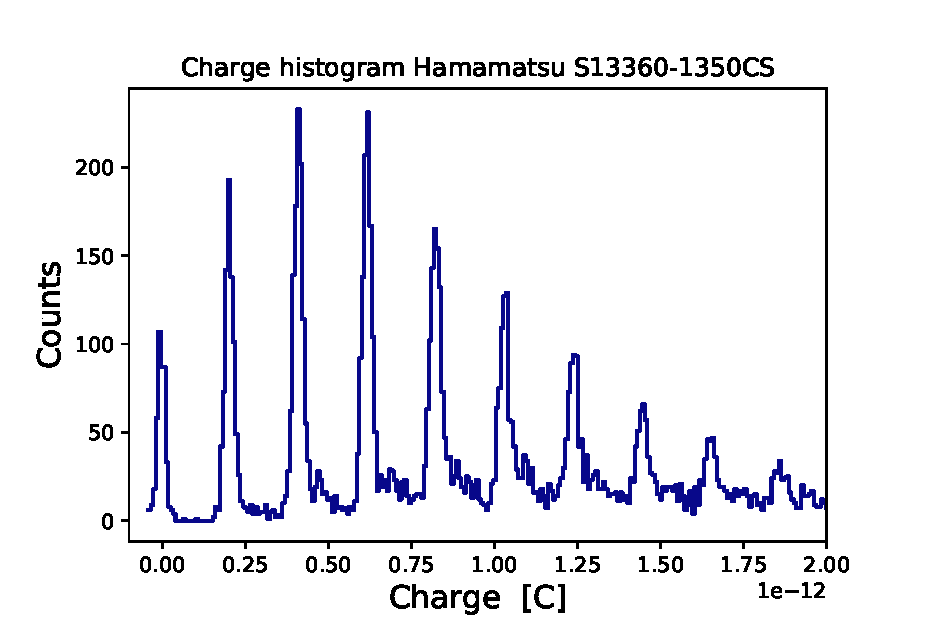
\includegraphics[scale=0.55]{Figures/Charge}
\caption{Pulsos generados por el SiPM 13360-1350CS a 25$^{\circ}$C y 56V (izquierda). Histograma de carga para el SiPM 13360-1350CS a 25$^{\circ}$C y 56V (derecha).}
\label{Charge}
\end{figure}

\subsubsection{Ganancia}

La ganancia del SiPM depende del voltaje de polarización, a medida que el voltaje aumenta, la ganancia también. Para determinar la ganancia del SiPM Hamamatsu 13360-1350CS se obtuvieron tres espectros p.e. para tres aumentos $\Delta$V del voltaje de polarización (1.7V[54V], 2.7V[55V], 3.7V[56V]) a 25$^{\circ}$C ($V_b$ = 52.3V). En la Fig. \ref{Gain}a se muestra la expansión de los espectros p.e. a medida que aumenta $\Delta$V debido al aumento de ganancia. \\

La ganancia se determina dividiendo la diferencia de carga entre picos $\Delta Q$ entre la carga de un electrón $e = 1.6 \times10^{19}$C. Para un $\Delta$V = 3.7V la ganancia es 1.3$\times10^6$ y el cambio de ganancia dependiendo del voltaje es 3.07$\times10^5$/V.

\begin{figure}[h!]
\centering
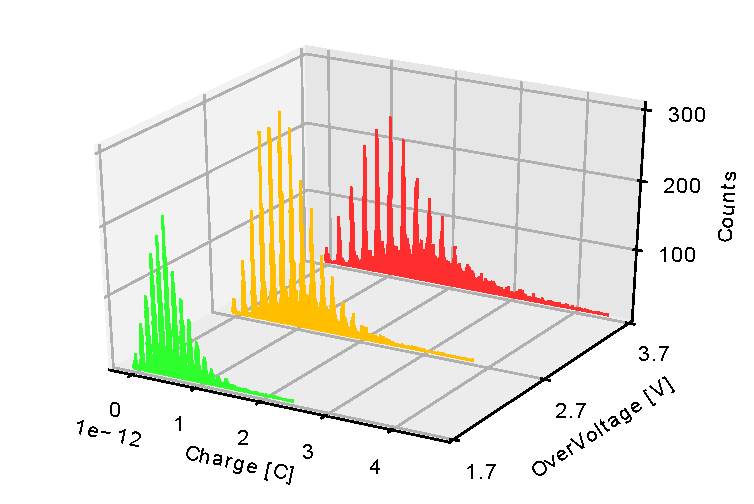
\includegraphics[scale=0.68]{Figures/GainCharge} 
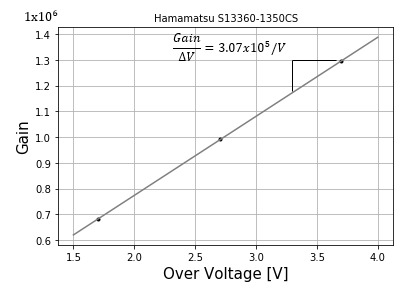
\includegraphics[scale=0.55]{Figures/Gain.jpeg}
\caption{Histograma de carga para el SiPM 13360-1350CS operando a tres sobre voltajes diferentes bajo las mismas condiciones de iluminación a 25$^{\circ}$C (izquierda). Ganancia en función del sobre voltaje a 25$^{\circ}$C (derecha). }
\label{Gain}
\end{figure}

\subsubsection{Conteo oscuro}

La principal fuente de ruido en el SiPM es el conteo oscuro (DCR). Este ocurre debido a electrones térmicamente generados que crean procesos de avalancha. Los pulsos eléctricos resultantes de este proceso son similares a las señales creadas por la incidencia de un fotón. La medición del DCR se debe realizar con el SiPM en condiciones de oscuridad.\\

En este caso, el DCR del SiPM 13360-1350CS se midió para diferentes valores umbrales de discriminación desde 0.1pe hasta 3.1pe a 25$^{\circ}$C como se muestra en la Fig. \ref{DCR}. Para un umbral de 0.5pe el DCR es $\sim$ 2$\times 10^5$ Hz correspondiendo con los valores esperados los cuales varían de 0.9$\times 10^5$ Hz a 2.7$\times 10^5$ Hz.\\

Por otra parte, el DCR disminuye drásticamente a medida que aumenta el nivel del umbral, siendo 1$\times 10^4$ Hz para 1.5pe y  8$\times 10^2$ Hz para 2.5pe. El efecto del DCR a 3.5pe es despreciable.

\begin{figure}[h!]
\centering
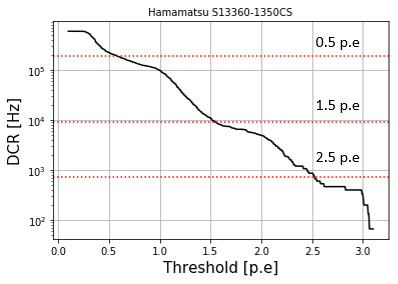
\includegraphics[scale=0.7]{Figures/DCR.jpeg} 
\caption{Frecuencia del conteo oscuro como función del umbral de conteo. }
\label{DCR}
\end{figure}
La prueba anterior permite establecer el valor mínimo que debe tener el umbral de detección de eventos en el sistema de adquisición con el fin de reducir la influencia del ruido por DCR.

\subsubsection{\textit{cross-talk} y \textit{after-pulse}}

Otro componente del ruido del SiPM es el \textit{crosstalk} y el \textit{afterpulse}. El \textit{crosstalk} ocurre cuando los portadores dentro de la avalancha emiten fotones que pueden interactuar con celdas vecinas dentro del SiPM, generando una avalancha en dicha celda. El \textit{crosstalk} se caracteriza por tener amplitudes de 2pe a 3pe.

\begin{figure}[h!]
\centering
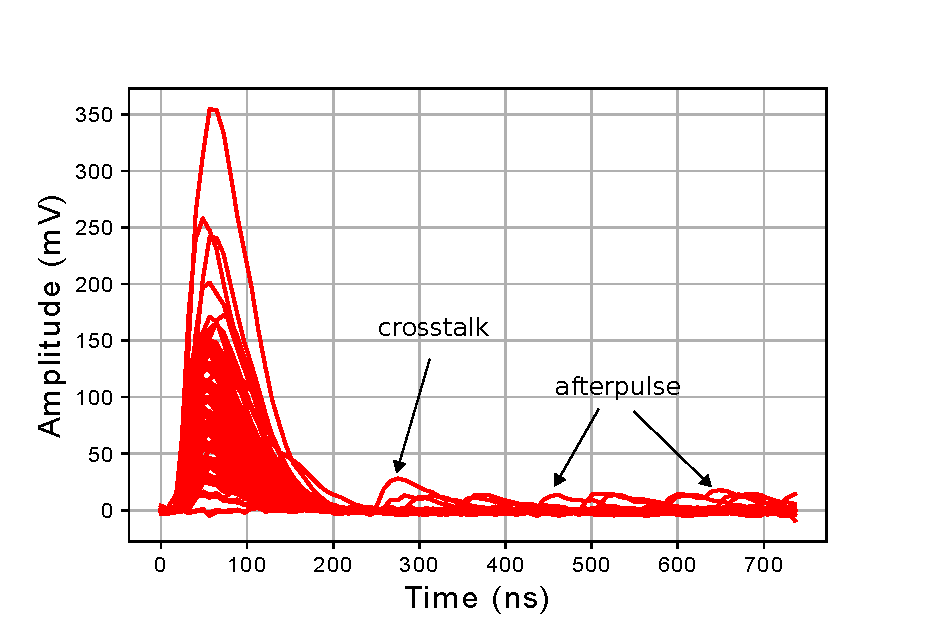
\includegraphics[scale=0.75]{Figures/After}
\caption{Pulsos característicos del \textit{cross-talk} (2pe) y \textit{after-pulse} (1pe) después de un pulso de estimulación lumínica. }
\label{cross}
\end{figure}

Por otra parte, el \textit{afterpulse} es generado por electrones que son atrapados en el material durante el desarrollo de la avalancha, estos electrones se liberan pocos nanosegundos después creando una nueva avalancha, y por ende un pulso consecutivo. En la Fig. \ref{cross} se muestra un ejemplo de \textit{crosstalk} y \textit{afterpulse}.

Para la estimación de estas dos fuentes de ruido se estimuló el SiPM mediante la fuente pulsada de luz a 500 Hz. En este caso el \textit{crosstalk} es $\sim$ 0.3$\%$ y el \textit{afterpulse} $\sim$ 3.4$\%$.

\subsection{Caracterización de las barras centelladoras}

El número de fotones que llegan al SiPM depende del lugar donde interactúa la partícula con el centellador \cite{Calderon2019}. Debido a la longitud de atenuación del centellador (5.5 cm) los fotones son canalizados hasta el SiPM a través de la fibra óptica.

\begin{figure}[h!]
\centering
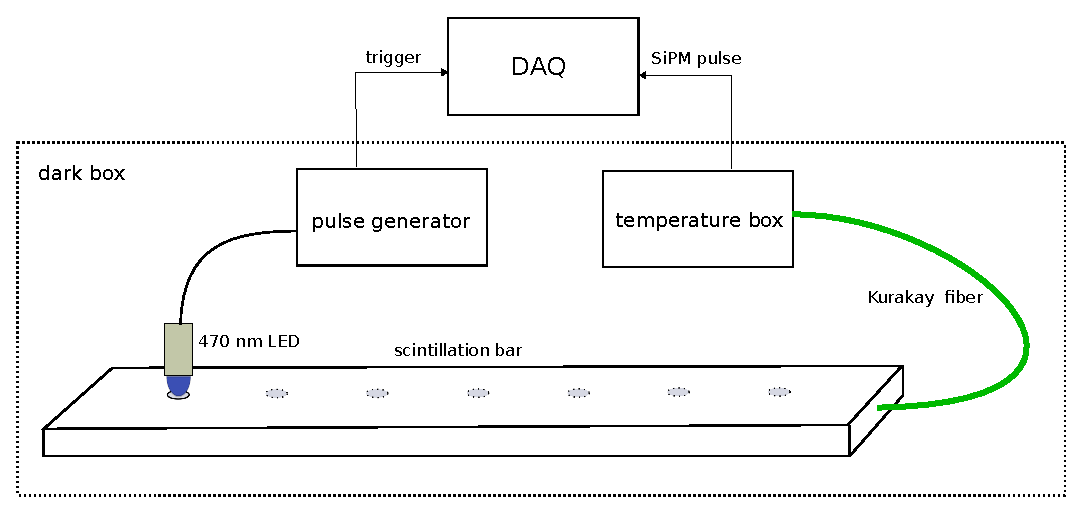
\includegraphics[scale=0.75]{Figures/BarAtt.eps}
\caption{Montaje experimental para la medición de la atenuación y el retardo en la señal registrada por los SiPM dependiendo de la distancia al punto de interacción en la barra centelladora.}
\label{AtTest}
\end{figure}

Para estimar la atenuación del sistema centellador-fibra, se crean 23 puntos de estimulación en el centellador con un paso de 5cm. Cada punto es estimulado con la fuente pulsada de 470nm. La señal generada por el SiPM es digitalizada a 14 bits y 125 MSPS. El montaje del experimento se muestra en la Fig. \ref{AtTest}.\\

Para cada punto de prueba se adquirieron 1000 puntos. A una distancia de x=120 cm la amplitud de la señal se atenúa hasta un 70$\%$ de la amplitud a x=0 cm. Dicho comportamiento de atenuación debe tenerse en cuenta durante la calibración de los paneles centelladores ya que en el píxel más alejado (x=120 cm, y=120 cm) de la zona donde se ubican los SiPM, la atenuación será 49$\%$.\\

Por otra parte, también se caracteriza el tiempo de retardo de la señal generada en el centellador dependiendo del punto de estimulación. Comparando tres puntos de estimulación en la barra centelladora (5 cm, 55 cm y 115 cm) se observa un retardo de 8.5 ns entre los puntos extremos ($\Delta x =$ 110 cm), es decir, los fotones recorren 1 cm en 77.2 ps. En la Fig. \ref{AttCur} se observan los tiempos de arribo de la señal al SiPM dependiendo del punto de interacción y la curva de atenuación del centellador.

\begin{figure}[h!]
\centering
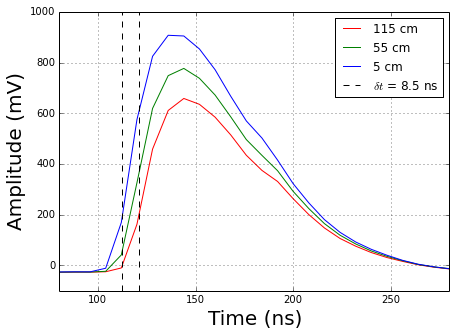
\includegraphics[scale=0.5]{Figures/arrivT.png}
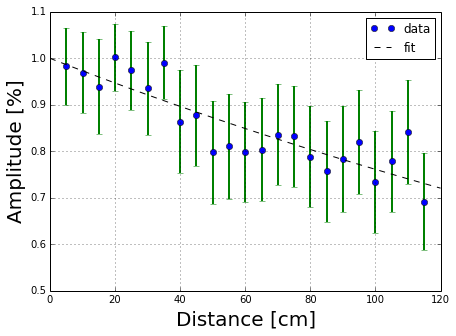
\includegraphics[scale=0.5]{Figures/Attenuation.png}
\caption{Retardo temporal de la señal del SiPM para una estimulación a 115 cm, 55 cm y 5 cm (izquierda). Curva de atenuación de la señal del SiPM dependiendo de la distancia de la estimulación (derecha).}
\label{AttCur}
\end{figure}

\subsection{Calibración de los paneles centelladores y hodoscopio}

El desempeño de los paneles centelladores es evaluado mediante el registro de flujo de muones atmosféricos. En este caso, los paneles registraron el flujo durante 15 horas continuas. Con los datos obtenidos se evaluó la varianza del flujo registrado por cada una de las 60 barras centelladores que componen cada panel. En la Fig. \ref{Bar_var} se observan los resultados obtenidos donde las barras detectan un promedio de 836 eventos/hora con una variabilidad de 96.3 eventos/h.

\begin{figure}[h!]
\centering
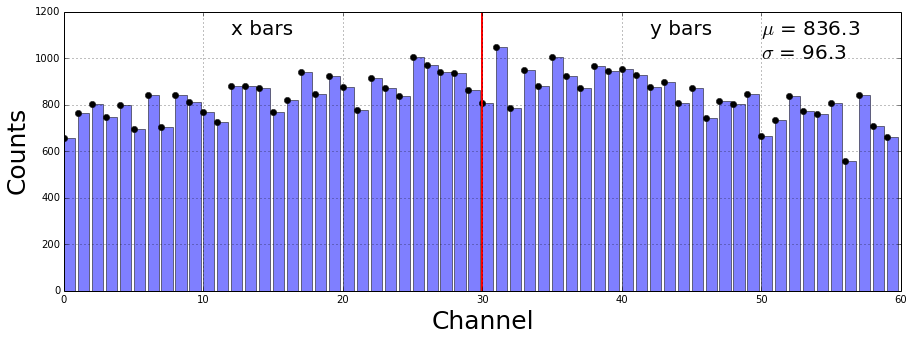
\includegraphics[scale=0.5]{Figures/hist2.png}
\caption{Histograma de eventos registrados por las 60 barras de un panel centellador durante una hora de registro. La línea roja separa las barras verticales y horizontales que componen la matriz de píxeles.}
\label{Bar_var}
\end{figure}

Por otra parte, los paneles centelladores presentan una atenuación debido a la combinación de la atenuación de las barras que lo componen. En la Fig. \ref{Pan_At} se muestra el histograma de conteo de los eventos registrados en 15 horas. En este caso, los píxeles más alejados (29,29) de la posición de los SiPM presentan un número de eventos menor en comparación al más cercano (0,0). La atenuación esperada en cada píxel se estima como la multiplicación de las atenuaciones de la barra-x y la barra-y que componen dicho píxel. El histograma de eventos en el panel permite además evaluar problemas en las barras centelladoras. En este caso podemos ver un mal funcionamiento de la barra-y 26 y 20.

\begin{figure}[h!]
\centering
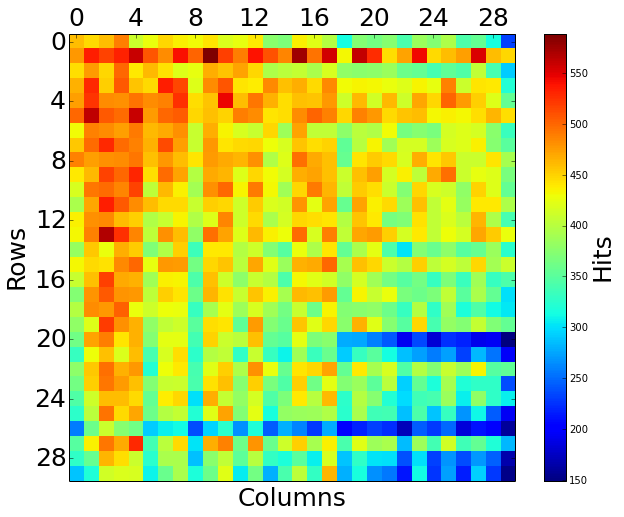
\includegraphics[scale=0.5]{Figures/P2_15h.png}
\caption{Histograma de eventos registrados por un panel centellador durante 15 horas. La atenuación del número de eventos registrados se incrementa diagonalmente desde la esquina superior-izquierda (0,0) a la esquina inferior-derecha (29,29).}
\label{Pan_At}
\end{figure}


\section{Diseño electrónico y calibración del WCD}

Para eliminar las fuentes de ruido que influyen en la técnica de muografía se emplearán sistemas de identificación de partículas. La diferenciación entre los eventos generados por la componente suave de las EAS (electrones y positrones) y los muones se realizará mediante la medición de la pérdida de energía de estas partículas cargadas en un WCD. El WCD de MuTe se diseñará y construirá teniendo en cuenta la experiencia previa del proyecto LAGO\footnote{http://lagoproject.net/} (por sus siglas en inglés Latin American Giant Observatory) del cual nuestro grupo hace parte.\\

Los detalles técnicos y resultados preliminares de las actividades relacionadas con este objetivo se muestran a continuación.\\

\textbf{Actividades y resultados preliminares}\\

\subsection{Diseño del WCD}

El WCD está compuesto por un tanque cúbico de aluminio con 120 cm de lado, recubierto internamente con Tyvek para aumentar la eficiencia en la detección de los fotones Cherenkov. El WCD esta lleno de agua purificada con 28 ppm de cloro. El dispositivo sensor es el tubo foto-multiplicador (PMT) Hamamatsu R5912 de 8". El PMT tiene una eficiencia cuática 22$\%$ a 390 nm, una ganancia de hasta 10$^7$ con un voltaje de polarización de 1800 V y un tiempo subida en el ánodo de 3.8 ns. La estructura del WCD se muestra en la Fig. \ref{WCD}.\\

\begin{figure}[h!]
\centering
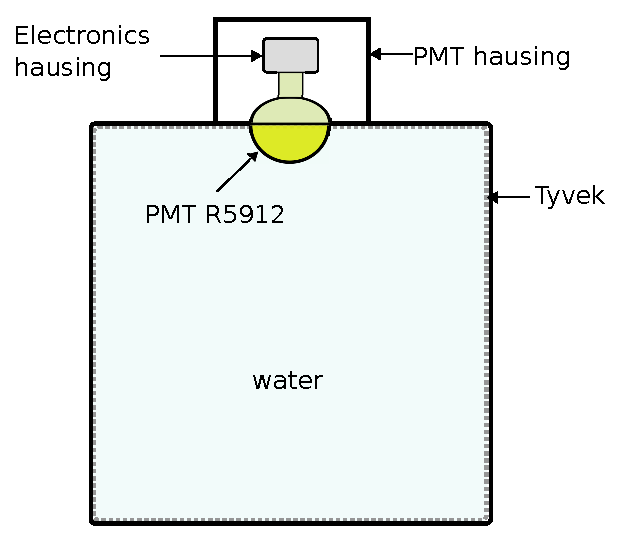
\includegraphics[scale=1]{Figures/WCD.eps}
\caption{Estructura mecánica del WCD de MuTe.}
\label{WCD}
\end{figure}

\subsection{Diseño del sistema de adquisición del WCD}

El sistema de adquisición del WCD registra las señales del ánodo y del último dínodo del PMT. Para aumentar el rango de medida la señal del dínodo es amplificada en un factor 20. La señales son digitalizadas por un ADC de 10 bits con una frecuencia de muestreo de 40 MHz. Cuando un evento supera el umbral de detección la forma de onda del pulso es almacenada en un vector de 12 muestras (300 ns).\\

Cada evento tiene una estampa temporal de 25 ns de resolución, la cual es sincronizada con la señal PPS del GPS. Los datos son transmitidos por protocolo UART a un SCB (Cubieboard II) que los almacena en archivos de una hora de registro junto con metadatos de temperatura y presión atmosférica.\\

Los eventos en coincidencia con el hodoscopio se registran a través de la señal de disparo (NIM Trigger). El esquema general del sistema de adquisición se muestra en la Fig. \ref{WCDDAQ}.

\begin{figure}[h!]
\centering
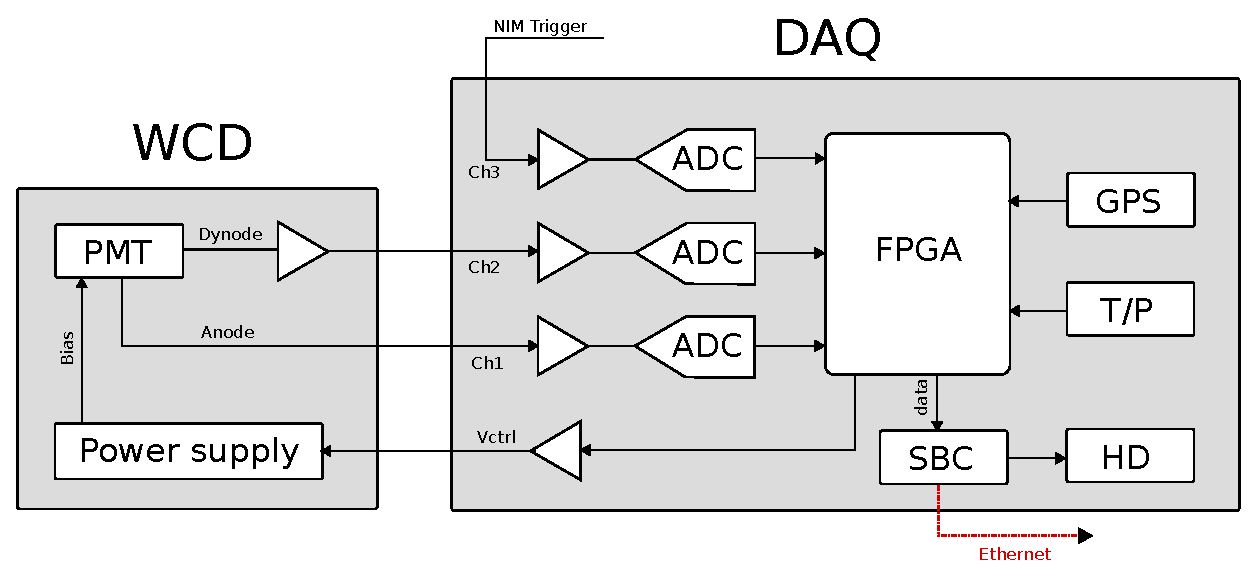
\includegraphics[scale=0.7]{Figures/WCDDAQ.eps}
\caption{Esquema general del sistema de adquisición del WCD}
\label{WCDDAQ}
\end{figure}

\subsection{Calibración del WCD}

La calibración del WCD se compone de dos pasos: la calibración del voltaje óptimo de operación del PMT y la calibración de la energía depositada por las partículas cargadas.\\

\subsubsection{Calibración del voltaje de polarización}

Para realizar la calibración del voltaje óptimo se registran la tasa de eventos $\Phi$ del fondo de rayos cósmicos a diferentes voltajes de polarización y diferentes umbrales de discriminación \cite{Leon2017}.\\

La calibración del WCD consistió en hacer un barrido de voltajes de polarización desde 740 V a 1450 V con pasos de 102 V para tres diferentes umbrales de discriminación: 110 mV, 160 mV y 210 mV. Para cada caso, se registraron 10 minutos de datos. En la Fig. \ref{plateau} se muestra la tasa de eventos registrados dependiendo del voltaje de polarización para 110 mV (negro), 160 mV (azul) y 210 mV(rojo).\\

En las curvas se puede observar una región de baja pendiente llamada \textit{plateau}. En esta región se ubica el punto óptimo de operación del PMT. Para hallar dicho punto se desarrolló un método automático que se basa en la minimización de la derivada respecto al voltaje de la tasa de detección.\\

Por lo tanto, el voltaje óptimo de operación $V^{\ast}_b$ es definido como:

\begin{equation}
V^{\ast}_b =  \textrm{argmin} \frac{\textrm{d}\Phi}{\textrm{d} V} 
\end{equation}

\begin{figure}[h!]
\begin{center}
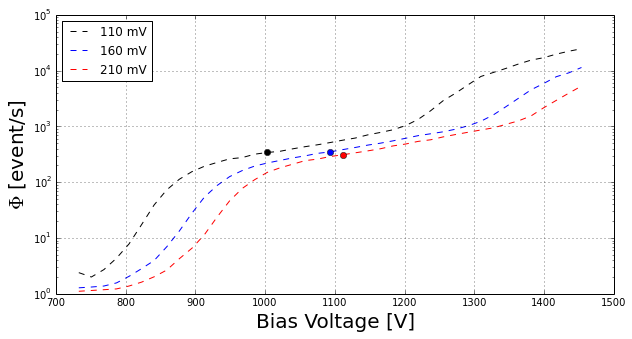
\includegraphics[width=0.8\textwidth]{Figures/WCDCalibrated}
\caption{Tasa de eventos detectada para voltajes de polarización desde 740 V hasta 1450 V para un umbral de 110 mV (negro), 160 mV (azul) y 210 mV (rojo).}
\label{plateau}
\end{center}
\end{figure}

\begin{figure}[h!]
\begin{center}
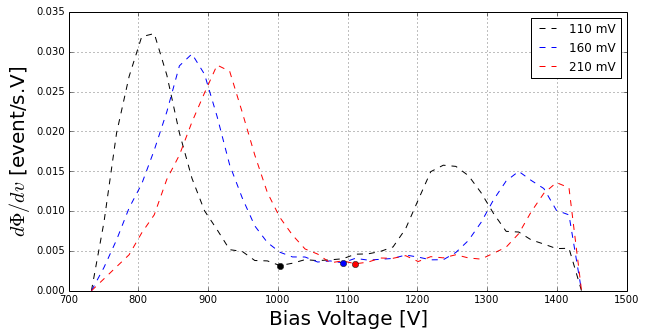
\includegraphics[width=0.8\textwidth]{Figures/OptimumPoint}
\caption{Voltaje óptimo de polarización del WCD para un umbral de 110 mV (negro), 160 mV (azul) y 210 mV (rojo).}
\label{OptimumWCD}
\end{center}
\end{figure}

En la Fig. \ref{OptimumWCD} se observan los voltajes de polarización hallados para los tres casos evaluados, 1000 V (110 mV), 1096 V (160 mV) y 1109 V (210 mV). 

\subsubsection{Calibración de la respuesta a la energía depositada}

Un punto importante es la calibración de la respuesta del WCD a la energía depositada de las partículas cargadas que lo atraviesan. Para ello se genera un histograma de carga desde los datos recolectados. Este histograma se basa en estimar el área bajo la curva de cada pulso registrado y sus unidades son ADC.bin.\\

En la Fig. \ref{ChargeHis} se muestra el histograma de carga para una hora de datos. Se pueden observar dos jorobas, la más pronunciada se debe a la componente electromagnética de las EAS, es decir, electrones, positrones y gammas. Por otra parte, la segunda joroba pertenece a la componente muónica de las EAS y su media se denomina VEM.\\

\begin{figure}[h!]
\begin{center}
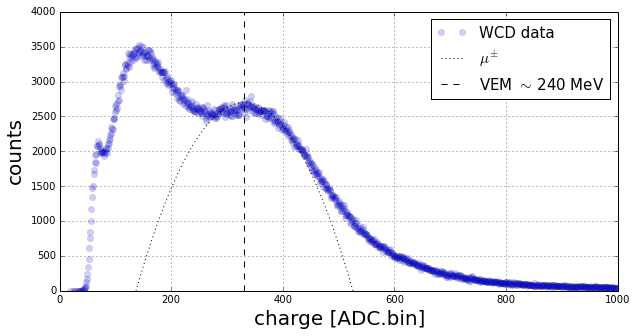
\includegraphics[width=0.8\textwidth]{Figures/dEdxCal}
\caption{Histograma de carga para una hora de datos. El VEM se ubica en 331.4 ADC.bin.}
\label{ChargeHis}
\end{center}
\end{figure}

El VEM (equivalente a un muón vertical) es la pérdida de energía que genera un muón cuando ingresa ortogonalmente por la parte superior del WCD. Teniendo en cuenta que un muón pierde alrededor de 2 MeV/cm en el agua, y que la altura del WCD es de 120 cm, entonces la pérdida de energía total de un muón que atraviese el WCD ortogonalmente es de 240 MeV.\\

Teniendo en cuenta lo anterior, la pérdida de energía dependiendo de la carga depositada se expresa como:

\begin{equation}
    E_{loss} =  (\text{ADC.bin})\frac{240 \text(MeV)}{ \text{VEM}_q(\text{ADC.bin})}
\end{equation}

donde $\text{VEM}_q$ es el valor del VEM en el histograma de carga, en este caso 331.4 ADC.bin.

\section{Diseño y calibración del sistema ToF}

Para filtrar los muones de baja energía ($<$ 1 GeV) \cite{Bozza2017} que componen una de las principales fuentes de contaminación en muografía se desarrollará un sistema de medición del tiempo de vuelo de las partículas cargadas que cruzan el hodoscopio. En este caso, se diseñará una arquitectura basada en líneas de retardo y un oscilador de anillo implementados en una FPGA Spartan 6 de Xilinx. Finalmente, el sistema ToF será calibrado y validado mediante la comparación de mediciones con el sistema ToF comercial TDC7200 de Texas Instruments.\\

Los detalles técnicos y resultados preliminares de las actividades relacionadas con este objetivo se muestran a continuación.\\

\textbf{Actividades y resultados preliminares}\\

\subsection{Diseño del sistema  TDC}

El sistema ToF se basa en un TDC (Time-to-Digital Converter) compuesto de una línea de retardo de 100 etapas (contador fino) y un oscilador de anillo para ampliar el rango de medición (contador grueso). Ver Fig. \ref{Arch}.\\

\begin{figure}[h!]
\begin{center}
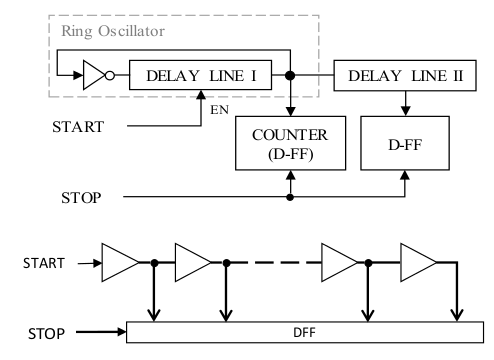
\includegraphics[width=0.6\textwidth]{Figures/Architecture}
\caption{Esquema del sistema de medición del tiempo de vuelo compuesto por una línea de retardo (contador fino) y un oscilador de anillo (contador grueso) (arriba). Esquema básico de la línea de retardo (abajo).}
\label{Arch}
\end{center}
\end{figure}

El TDC se implemento en una FPGA Spartan 6. Las etapas de retardo se diseñaron usando el módulo CARRY4 el cual está compuesto de 4 multiplexores los cuales se ubicaron de manera consecutiva para garantizar una respuesta lineal del TDC.\\

\subsection{Calibración del sistema  TDC}

La calibración del contador fino se realizó inyectando una señal cuadrada de 200 Hz desde un generador de señales (Tektronix AFG1022) y observando su retraso después de pasar secciones de 10 etapas. La curva de calibración obtenida se puede ver en la Fig. \ref{loc}. El retardo promedio por etapa es de 40$\pm$26 ps.\\

\begin{figure}[h!]
\begin{center}
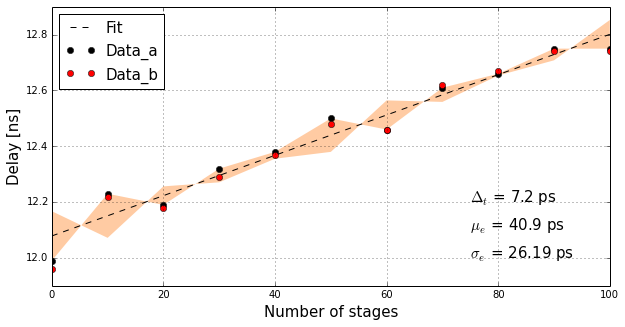
\includegraphics[width=0.7\textwidth]{Figures/ToF_delay}
\caption{Retardo de la señal dependiendo del número de etapas ubicadas en dos regiones distintas de la FPGA (a y b)}
\label{loc}
\end{center}
\end{figure}

El contador grueso se compone de una línea de retardo de 100 etapas retroalimentada con el inverso de su salida. La retroalimentación es controlada a través de un multiplexor.

\begin{figure}[h!]
\begin{center}
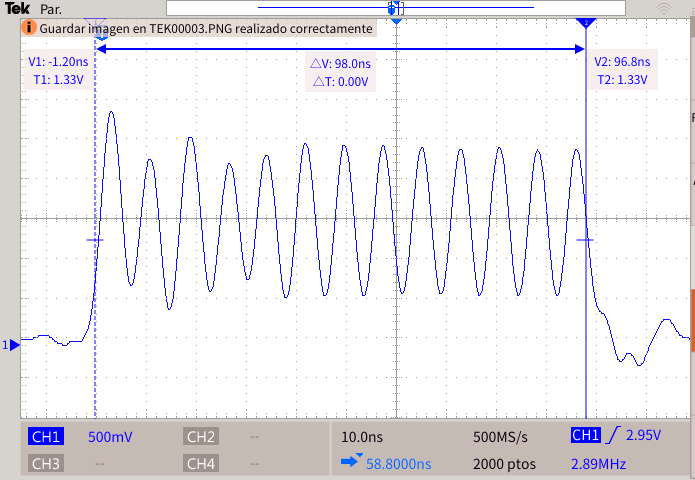
\includegraphics[width=0.6\textwidth]{Figures/Ringwaves}
\caption{Salida del oscilador de anillo para un retraso entre la señal \textbf{Start} y \textbf{Stop} de 100 ns.}
\label{waves}
\end{center}
\end{figure}

Teniendo que cada etapa tiene un retardo de 40$\pm$26 ps, el período de oscilación esperado para 100 etapas es $\sim$8 ns. En la Fig. \ref{waves} se muestra la salida del oscilador de anillo para un retrazo entre la señal \textbf{Start} y \textbf{Stop} de 100 ns. En este caso, se registran 13 oscilaciones, es decir, el periodo de oscilación es $\sim$7.7ns.\\



Para calibrar el contador grueso se ingresaron retardos controlados desde 0 ns a 90 ns medidos paralelamente con un osciloscopio Textronix TDS2004B. En la Fig. \ref{CalCoarse} se muestra el conteo de los picos de oscilación dependiendo del tiempo de retardo entre \textbf{Start} y \textbf{Stop}. La linealidad de la etapa disminuye a medida que el rango de medición aumenta, la región óptima de medición se ubica de 0 ns a 60 ns. Además, el desempeño del sistema TDC implementado en MuTe será comparado con el TDC7200 de Texas Instruments.

\begin{figure}[h!]
\begin{center}
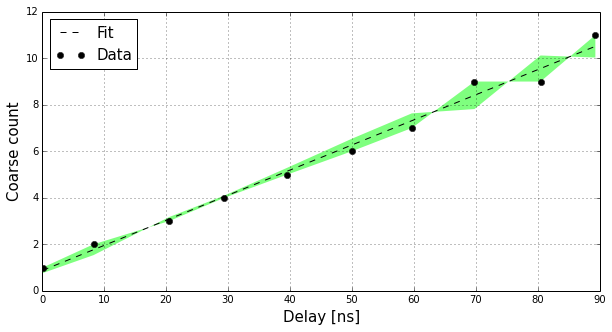
\includegraphics[width=0.7\textwidth]{Figures/Cal_coarse}
\caption{Curva de calibración del contador grueso del sistema ToF.}
\label{CalCoarse}
\end{center}
\end{figure}

Los datos del ToF se transmiten a la SBC de cada panel mediante un protocolo I2C en una trama compuesta por dos valores: el contador fino y el contador grueso.

\section{Calibración del MuTe y pruebas de estabilidad}

Una vez se calibra el hodoscopio y el WCD, se procederá a la calibración conjunta del MuTe. La calibración se hará mediante la detección de eventos provenientes del fondo de rayos cósmicos atmosféricos y el análisis de datos.\\

El MuTe registrará eventos continuamente durante varios días junto con los metadatos de temperatura, presión atmosférica, consumo eléctrico y estampas temporales de los paneles centelladores y el WCD. Los datos serán analizados evaluando los siguientes aspectos:

\begin{itemize}
    \item Funcionamiento total de las barras centelladoras en busca de fallas por transporte
    \item Posibles variaciones del flujo registrado por los paneles de centelleo y el WCD debido a variaciones de temperatura o presión atmosférica
    \item Excesos en el pico electromagnético del WCD debido a contaminación por fotones
    \item Correcta transmisión de los datos desde los paneles de centelleo al disco duro central
    \item Evaluación de coincidencias entre el hodoscopio y el WCD
    \item Corrección temporal de los eventos teniendo en cuenta los retrasos por las líneas de transmisión
    \item Imágenes muongráficas con y sin las componentes generadoras de ruido
    
\end{itemize}

Finalmente, el detector se dejará adquiriendo de manera constante hasta que se necesite trasladar a otro sitio.

%\input{Plan/Plan}
\chapter{Cronograma}

%\begin{adjustbox}{angle=90}
\begin{tabular}{|l|c|c|c|c|c|c|c|c|c|c|c|c|} \hline
\multirow{3}{*}{\textbf{Actividad}} & \multicolumn{12}{ c| }{\textbf{Año}}	\\  \cline{2-13}

\multirow{3}{*}{} & \multicolumn{3}{ c| }{2017} & \multicolumn{3}{ c| }{2018} & \multicolumn{3}{ c| }{2019} & \multicolumn{3}{ c| }{2020}	\\  \cline{2-13}

\multirow{3}{*}{} & \multicolumn{12}{ c| }{Cuatrimestre}	\\\hline

%				           & 1 & 2 & 3 & 4 & 5 & 6 & 7 & 8 & 9 & 10 & 11 & 12 \\\hline
				           
Cursos & \cellcolor{green!25} & \cellcolor{green!25} & \cellcolor{green!25} & \cellcolor{green!25} &  &  &  &  &  &  & & \\\hline
\textbf{Revisión bibliográfica} &  \cellcolor{red!50} &\cellcolor{red!50}& \cellcolor{red!50}&  & \cellcolor{red!25}&  &\cellcolor{red!25} & & \cellcolor{red!25} &  & \cellcolor{red!25} & \\\hline
Monografía &   &  &  & \cellcolor{green!25} & \cellcolor{green!25}  &   &   &   &   &   &   & \\\hline
Propuesta &   &  &  &   &   & \cellcolor{green!25} & \cellcolor{blue!25}     &   &   &   &   & \\\hline

\multirow{1}{*}{\textbf{Diseño y construcción hodoscopio}} & \multicolumn{12}{ c| }{}	\\ \hline
Barras centelladoras y SiPM	& & \cellcolor{green!25}& \cellcolor{green!25}  & & & & & & & & & \\\hline
Sistema de adquisición 	& & & \cellcolor{green!25} & \cellcolor{green!25} & \cellcolor{green!25} & \cellcolor{green!25} & & & & & &   \\\hline
Sistema de control 	& & & & \cellcolor{green!25} & \cellcolor{green!25} & \cellcolor{green!25} & & & & &   &   \\\hline
Sistema ToF	& & & & \cellcolor{green!25}  & \cellcolor{green!25}  & & & & & & &  \\\hline
Sistema de disparo & & & & & \cellcolor{green!25}  & \cellcolor{green!25} & & & & & &   \\\hline
Periféricos	& & & & & \cellcolor{green!25}  & \cellcolor{green!25} & & & & & &   \\\hline

\multirow{1}{*}{\textbf{Calibración hodoscopio}} & \multicolumn{12}{ c| }{}	\\ \hline
Caracterización del SiPM & & & \cellcolor{green!25}& & & & & & & & & \\\hline
%Caracterización barra centelladora  & & & & \cellcolor{green!25} & & & & & & & &  \\\hline
Paneles centelladores  & & & & & \cellcolor{green!25} & \cellcolor{green!25} & & & & & &  \\\hline
Calibración del ToF	& & & & & \cellcolor{green!25} & \cellcolor{green!25} & \cellcolor{blue!25}& & & & &  \\\hline
Sistema de disparo	& & & & & \cellcolor{green!25} & \cellcolor{green!25} &\cellcolor{green!25} & \cellcolor{blue!25}& & & &  \\\hline

\multirow{1}{*}{\textbf{Detector Cherenkov}} & \multicolumn{12}{ c| }{}	\\ \hline
Construcción del WCD & & & & & & & \cellcolor{green!25}  & \cellcolor{green!25}  & & & & \\\hline
Calibración del WCD	& & & & & & & & \cellcolor{green!25}&  \cellcolor{green!25} &  & & \\\hline

\multirow{1}{*}{\textbf{MuTe}} & \multicolumn{12}{ c| }{}	\\ \hline
Instalación de MuTe	& & & & & & & & & \cellcolor{green!25} & \cellcolor{blue!25} &  & \\\hline

\textbf{Escritura del libro y resultados} &  & & &  & \cellcolor{red!25}&  &\cellcolor{red!25} & & \cellcolor{red!25} &  & \cellcolor{red!25} & \cellcolor{red!25} \\\hline

\end{tabular}
\\ \\
\textcolor{red}{Ejecución continua}\\
\textcolor{green}{Ejecutado}\\
\textcolor{blue}{En ejecución}

%\end{adjustbox}
\chapter{Presupuesto}

\section{Recursos humanos}

\begin{tabular}{|c|c|c|c|}\hline
{\bf Item} 	& {\bf Descripción} 			& {\bf Dedicación} 	& {\bf Costo (COP)} \\
                                            &	    & {\bf H/Sem}  & 	\\\hline
Estudiante 	        &  Beca Colciencias		&  40   & 				\\
de doctorado  	    &  durante 4 años		&       & 144.000.000     	\\\hline

Director del 	    & Horas de asesoría		& 2	    & 20.000.000  		\\
Proyecto  		    & 		                &  		& 				\\\hline
Codirector 	        & Horas de asesoría 	& 1     & 10.000.000  		\\
del Proyecto        &  	                    & 		& 		\\\hline
\multicolumn{3}{|c|}{\bf Costo Total} 	    & {\bf 174.000.000}			\\\hline
\end{tabular}


\section{Materiales}

\begin{tabular}{|c|c|c|}\hline
{\bf Item} 	& Cantidad & {\bf Costo (COP)} \\
		   & & \\\hline
Barras centelladoras Fermilab 	&  130 & 6.000.000 	\\
(Down Styron 663) &   & 	\\\hline
Fibra óptica (Saint-Gobain BCF-92)	        &  160 m & 2.000.000 	\\\hline
SiPM (Hamamatsu S13360-1350CS)	                &  130 & 5.000.000 	\\\hline
Cable coaxial	(RG178U)      &  200 m & 2.000.000 	\\\hline
Sistema adquisición	(MAROC3A)    &  2 & 3.000.000 	\\\hline
Sistema de control	    &  2 & 2.000.000 	\\\hline
Sistema ToF	            &  2 & 1.000.000 	\\\hline
Periféricos	            &  2 & 1.000.000 	\\\hline
Fotomultiplicador (Hamamatsu R5912)	    &  1 & 6.000.000 	\\\hline
Discos duros	        &  2 & 2.000.000 	\\\hline
Estructura mecánica     &  1    & 20.000.000 \\\hline
\multicolumn{2}{|c|}{\bf Costo Total} 						          & {\bf 50.000.000}					\\\hline
\end{tabular}

Las pruebas de caracterización de las barras centelladoras y SiPM se realizaron como parte del proyecto de pregrado 
\textbf{Diseño e implementación de un sistema para la caracterización de los SiPM del Telescopio de Muones (MuTe)} \cite{Villafrades2019} y la tesis de maestría \textbf{Estudio de centelladores plásticos en el proyecto MuTe para muongrafía de volcanes} \cite{Calderon2019}.

\section{Equipos}

Las especificaciones de los equipos requeridos se muestran en la siguiente tabla.\\

\begin{tabular}{|c|c|c|}\hline
{\bf Item} 	& Cantidad & {\bf Costo (COP)} \\
		   & & \\\hline
Computador portátil	    &  1 & 3.000.000 	\\\hline
Osciloscopio    &  1 & 4.000.000 	\\
(Tektronix TBS 2000 - 1 GS/s - 4 CH) & & \\\hline
Generador de señales 	&  1 & 3.000.000 	\\
(Tektronix AFG1022 -  125 MS/s)	&   & 	\\\hline
Caja oscura	            &  1 & 1.000.000 	\\\hline
Sistema de control de T$^{\circ}$	&  1 & 1.000.000 	\\\hline
Red Pitaya (125 MS/s)              &  2 & 500.000 	\\\hline
Fuente de pulsos LED (FWHM 9 ns)              & 1 & 400.000 	\\\hline
Multímetro UNIT 61C            &  2 & 500.000 	\\\hline
\multicolumn{2}{|c|}{\bf Costo Total} 						          & {\bf 12.900.000}					\\\hline
\end{tabular}\\

Los equipos requeridos en este proyecto deben cumplir con algunas especificaciones. El osciloscopio debe muestrear señales de hasta 100 MHz además de medir simultáneamente varios canales para analizar el retraso de señales de disparo y tiempos de ocurrencia. La caja de temperatura debe proporcionar un sistema controlado que mantenga la temperatura de los SiPM a un valor establecido entre 0$^{\circ}$C hasta 60$^{\circ}$C.\\

La fuente de pulsos LED debe generar pulsos lumínicos a 470 nm con frecuencias variables de 100 Hz hasta decenas de KHz y anchos de pulso (FWHM) menores a 10 ns. \\

Finalmente, el sistema de registro de pulsos debe tener una frecuencia de muestreo $>$ 100 MHz y una resolución temporal capaz de medir la cuantización de la amplitud de los SiPM (1 UADC $<$ 20 mV). 

\section{Costo Total del Proyecto}

\begin{tabular}{|c|c|}\hline
{\bf Item} & {\bf Costo} \\
			& 				\\\hline
Recursos humanos	&  174.000.000 \\\hline
Materiales			& 50.000.000	\\\hline
Equipos			& 12.500.000	\\\hline
\bf Costo Total		  			& {\bf 236.500.000}		\\\hline
\end{tabular}

\vspace{2cm}

* El costo de equipos y materiales serán cubiertos por Colciencias a través del proyecto \textbf{Telescopio de Muones para Muongrafía Volcánica, MuTe} con código \textbf{110266044583} y número de contrato \textbf{FP44842-082-2015}.\\

** Los recursos humanos mencionados aquí son los implicados en este trabajo de investigación, no en la totalidad del proyecto \textbf{MuTe}.

%\chapter{Trabajo actual}
%\chapter{Conclusiones}

\newpage
%%%%%%%%%%%%%%%%%%%%%%%%% Bibliografia %%%%%%%%%%%%%%%%%%%%%5
\cleardoublepage
\addcontentsline{toc}{chapter}{Bibliografía}%para que aparezca en la tabla de contenidos
\bibliographystyle{unsrt}
\bibliography{Bibliography/MuTe.bib}
%Archivo con las referencias bibliográficas, creado en JabRef (o manualmente)

\end{document}
